%% Преамбула TeX-файла

% 1. Стиль и язык
\documentclass[utf8x, 14pt]{G7-32} % Стиль (по умолчанию будет 14pt)

\newgeometry{left=30mm, right=10mm, top=20mm, bottom=20mm}
% Остальные стандартные настройки убраны в preamble.inc.tex.
\sloppy

% Настройки стиля ГОСТ 7-32
% Для начала определяем, хотим мы или нет, чтобы рисунки и таблицы нумеровались в пределах раздела, или нам нужна сквозная нумерация.
\EqInChapter % формулы будут нумероваться в пределах раздела
\TableInChapter % таблицы будут нумероваться в пределах раздела
\PicInChapter % рисунки будут нумероваться в пределах раздела

% Добавляем гипертекстовое оглавление в PDF
\usepackage[
bookmarks=true, colorlinks=true, unicode=true,
urlcolor=black,linkcolor=black, anchorcolor=black,
citecolor=black, menucolor=black, filecolor=black,
]{hyperref}

\AfterHyperrefFix

\usepackage{microtype}% полезный пакет для микротипографии, увы под xelatex мало чего умеет, но под pdflatex хорошо улучшает читаемость

% Тире могут быть невидимы в Adobe Reader
\ifInvisibleDashes
\MakeDashesBold
\fi

\usepackage{graphicx}   % Пакет для включения рисунков

% С такими оно полями оно работает по-умолчанию:
% \RequirePackage[left=20mm,right=10mm,top=20mm,bottom=20mm,headsep=0pt,includefoot]{geometry}
% Если вас тошнит от поля в 10мм --- увеличивайте до 20-ти, ну и про переплёт не забывайте:
\geometry{right=20mm}
\geometry{left=30mm}
\geometry{bottom=20mm}
\geometry{ignorefoot}% считать от нижней границы текста

\usepackage{color} %use color
\definecolor{mygreen}{rgb}{0,0.6,0}
\definecolor{mygray}{rgb}{0.5,0.5,0.5}
\definecolor{mymauve}{rgb}{0.58,0,0.82}

\usepackage{listings} %% собственно, это и есть пакет listings
\renewcommand{\lstlistingname}{Листинг}
%%
%% GLSL definition (c) 2020 Benno Bielmeier
%%
\lstdefinelanguage{GLSL}%
{%
	morekeywords={%
	% HLSL constants
		false,FALSE,NULL,true,TRUE,%
	% GLSL predefinde macro constant
		__LINE__,__FILE__,__VERSION__,GL_core_profile,GL_es_profile,GL_compatibility_profile,%
	% GLSL precision modifier
		precision,highp,mediump,lowp,%
	% GLSL control keywords
		break,case,continue,default,discard,do,else,for,if,return,switch,while,%
	% GLSL types
		void,bool,int,uint,float,double,vec2,vec3,vec4,dvec2,dvec3,dvec4,bvec2,bvec3,bvec4,ivec2,ivec3,ivec4,uvec2,uvec3,uvec4,mat2,mat3,mat4,mat2x2,mat2x3,mat2x4,mat3x2,mat3x3,mat3x4,mat4x2,mat4x3,mat4x4,dmat2,dmat3,dmat4,dmat2x2,dmat2x3,dmat2x4,dmat3x2,dmat3x3,dmat3x4,dmat4x2,dmat4x3,dmat4x4,sampler1D,sampler2D,sampler3D,image1D,image2D,image3D,samplerCube,imageCube,sampler2DRect,image2DRect,sampler1DArray,sampler2DArray,image1DArray,image2DArray,samplerBuffer,imageBuffer,sampler2DMS,image2DMS,sampler2DMSArray,image2DMSArray,samplerCubeArray,imageCubeArray,sampler1DShadow,sampler2DShadow,sampler2DRectShadow,sampler1DArrayShadow,sampler2DArrayShadow,samplerCubeShadow,samplerCubeArrayShadow,isampler1D,isampler2D,isampler3D,iimage1D,iimage2D,iimage3D,isamplerCube,iimageCube,isampler2DRect,iimage2DRect,isampler1DArray,isampler2DArray,iimage1DArray,iimage2DArray,isamplerBuffer,iimageBuffer,isampler2DMS,iimage2DMS,isampler2DMSArray,iimage2DMSArray,isamplerCubeArray,iimageCubeArray,atomic_uint,usampler1D,usampler2D,usampler3D,uimage1D,uimage2D,uimage3D,usamplerCube,uimageCube,usampler2DRect,uimage2DRect,usampler1DArray,usampler2DArray,uimage1DArray,uimage2DArray,usamplerBuffer,uimageBuffer,usampler2DMS,uimage2DMS,usampler2DMSArray,uimage2DMSArray,usamplerCubeArray,uimageCubeArray,struct,%
	% GLSL support variables
		gl_BackColor,gl_BackLightModelProduct,gl_BackLightProduct,gl_BackMaterial,gl_BackSecondaryColor,gl_ClipDistance,gl_ClipPlane,gl_ClipVertex,gl_Color,gl_DepthRange,gl_DepthRangeParameters,gl_EyePlaneQ,gl_EyePlaneR,gl_EyePlaneS,gl_EyePlaneT,gl_Fog,gl_FogCoord,gl_FogFragCoord,gl_FogParameters,gl_FragColor,gl_FragCoord,gl_FragData,gl_FragDepth,gl_FrontColor,gl_FrontFacing,gl_FrontLightModelProduct,gl_FrontLightProduct,gl_FrontMaterial,gl_FrontSecondaryColor,gl_InstanceID,gl_Layer,gl_LightModel,gl_LightModelParameters,gl_LightModelProducts,gl_LightProducts,gl_LightSource,gl_LightSourceParameters,gl_MaterialParameters,gl_ModelViewMatrix,gl_ModelViewMatrixInverse,gl_ModelViewMatrixInverseTranspose,gl_ModelViewMatrixTranspose,gl_ModelViewProjectionMatrix,gl_ModelViewProjectionMatrixInverse,gl_ModelViewProjectionMatrixInverseTranspose,gl_ModelViewProjectionMatrixTranspose,gl_MultiTexCoord0,gl_MultiTexCoord1,gl_MultiTexCoord2,gl_MultiTexCoord3,gl_MultiTexCoord4,gl_MultiTexCoord5,gl_MultiTexCoord6,gl_MultiTexCoord7,gl_Normal,gl_NormalMatrix,gl_NormalScale,gl_ObjectPlaneQ,gl_ObjectPlaneR,gl_ObjectPlaneS,gl_ObjectPlaneT,gl_Point,gl_PointCoord,gl_PointParameters,gl_PointSize,gl_Position,gl_PrimitiveIDIn,gl_ProjectionMatrix,gl_ProjectionMatrixInverse,gl_ProjectionMatrixInverseTranspose,gl_ProjectionMatrixTranspose,gl_SecondaryColor,gl_TexCoord,gl_TextureEnvColor,gl_TextureMatrix,gl_TextureMatrixInverse,gl_TextureMatrixInverseTranspose,gl_TextureMatrixTranspose,gl_Vertex,gl_VertexID,%
	% GLSL support constants
		gl_MaxClipPlanes,gl_MaxCombinedTextureImageUnits,gl_MaxDrawBuffers,gl_MaxFragmentUniformComponents,gl_MaxLights,gl_MaxTextureCoords,gl_MaxTextureImageUnits,gl_MaxTextureUnits,gl_MaxVaryingFloats,gl_MaxVertexAttribs,gl_MaxVertexTextureImageUnits,gl_MaxVertexUniformComponents,%
	% GLSL support functions
		abs,acos,all,any,asin,atan,ceil,clamp,cos,cross,degrees,dFdx,dFdy,distance,dot,equal,exp,exp2,faceforward,floor,fract,ftransform,fwidth,greaterThan,greaterThanEqual,inversesqrt,length,lessThan,lessThanEqual,log,log2,matrixCompMult,max,min,mix,mod,noise1,noise2,noise3,noise4,normalize,not,notEqual,outerProduct,pow,radians,reflect,refract,shadow1D,shadow1DLod,shadow1DProj,shadow1DProjLod,shadow2D,shadow2DLod,shadow2DProj,shadow2DProjLod,sign,sin,smoothstep,sqrt,step,tan,texture1D,texture1DLod,texture1DProj,texture1DProjLod,texture2D,texture2DLod,texture2DProj,texture2DProjLod,texture3D,texture3DLod,texture3DProj,texture3DProjLod,textureCube,textureCubeLod,transpose,%
	% GLSL struct member -> FixMe: Should have dot(.) as delimiter
		rgb
	},
	sensitive=true,%
	comment=[l]{//},
	morecomment=[s]{/*}{*/},%
	morecomment=[l]//,%
    commentstyle=\color{purple}\ttfamily,
	stringstyle=\color{red}\ttfamily,
	morestring=[b]",%
	morestring=[b]',%
	moredelim=*[directive]\#,%
	% keyword.control.hlsl
	moredirectives={define,defined,elif,else,if,ifdef,endif,line,error,ifndef,include,pragma,undef,warning,extension,version}%
}[keywords,comments,strings,directives]%


\lstset{ %
	backgroundcolor=\color{white}, % choose the background color; you must add \usepackage{color} or \usepackage{xcolor}
	basicstyle=\footnotesize, % the size of the fonts that are used for the code
	breakatwhitespace=false, % sets if automatic breaks should only happen at whitespace
	breaklines=true, % sets automatic line breaking
	captionpos=t, % sets the caption-position to bottom
	commentstyle=\color{mygreen}, % comment style
	deletekeywords={...}, % if you want to delete keywords from the given language
	escapeinside={\%*}{*)}, % if you want to add LaTeX within your code
	extendedchars=true, % lets you use non-ASCII characters; for 8-bits encodings only, does not work with UTF-8
	frame=single, % adds a frame around the code
	keepspaces=true, % keeps spaces in text, useful for keeping indentation of code (possibly needs columns=flexible)
	keywordstyle=\color{blue}, % keyword style
	% language=Octave, % the language of the code
	morekeywords={*,...}, % if you want to add more keywords to the set
	numbers=left, % where to put the line-numbers; possible values are (none, left, right)
	numbersep=5pt, % how far the line-numbers are from the code
	numberstyle=\tiny\color{mygray}, % the style that is used for the line-numbers
	rulecolor=\color{black}, % if not set, the frame-color may be changed on line-breaks within not-black text (e.g. comments (green here))
	showspaces=false, % show spaces everywhere adding particular underscores; it overrides 'showstringspaces'
	showstringspaces=false, % underline spaces within strings only
	showtabs=false, % show tabs within strings adding particular underscores
	stepnumber=1, % the step between two line-numbers. If it's 1, each line will be numbered
	stringstyle=\color{mymauve}, % string literal style
	tabsize=2, % sets default tabsize to 2 spaces
	title=\lstname % show the filename of files included with \lstinputlisting; also try caption instead of title
}
%END of listing package%

% Пакет Tikz
\usepackage{tikz}
\usetikzlibrary{arrows,positioning,shadows}

% Произвольная нумерация списков.
\usepackage{enumerate}

% ячейки в несколько строчек
\usepackage{multirow}

% itemize внутри tabular
\usepackage{paralist,array}

%\setlength{\parskip}{1ex plus0.5ex minus0.5ex} % разрыв между абзацами
\setlength{\parskip}{1ex} % разрыв между абзацами
\usepackage{blindtext}

% Центрирование подписей к плавающим окружениям
%\usepackage[justification=centering]{caption}

\usepackage{newfloat}
\DeclareFloatingEnvironment[
placement={!ht},
name=Equation
]{eqndescNoIndent}
\edef\fixEqndesc{\noexpand\setlength{\noexpand\parindent}{\the\parindent}\noexpand\setlength{\noexpand\parskip}{\the\parskip}}
\newenvironment{eqndesc}[1][!ht]{%
    \begin{eqndescNoIndent}[#1]%
\fixEqndesc%
}
{\end{eqndescNoIndent}}


\usepackage{algorithm}
\usepackage{algpseudocode}



% Настройки листингов.
\ifPDFTeX
% 8 Листинги

\usepackage{listings}

% Значения по умолчанию
\lstset{
  basicstyle= \footnotesize,
  breakatwhitespace=true,% разрыв строк только на whitespacce
  breaklines=true,       % переносить длинные строки
%   captionpos=b,          % подписи снизу -- вроде не надо
  inputencoding=koi8-r,
  numbers=left,          % нумерация слева
  numberstyle=\footnotesize,
  showspaces=false,      % показывать пробелы подчеркиваниями -- идиотизм 70-х годов
  showstringspaces=false,
  showtabs=false,        % и табы тоже
  stepnumber=1,
  tabsize=4,              % кому нужны табы по 8 символов?
  frame=single
}

% Стиль для псевдокода: строчки обычно короткие, поэтому размер шрифта побольше
\lstdefinestyle{pseudocode}{
  basicstyle=\small,
  keywordstyle=\color{black}\bfseries\underbar,
  language=Pseudocode,
  numberstyle=\footnotesize,
  commentstyle=\footnotesize\it
}

% Стиль для обычного кода: маленький шрифт
\lstdefinestyle{realcode}{
  basicstyle=\scriptsize,
  numberstyle=\footnotesize
}

% Стиль для коротких кусков обычного кода: средний шрифт
\lstdefinestyle{simplecode}{
  basicstyle=\footnotesize,
  numberstyle=\footnotesize
}

% Стиль для BNF
\lstdefinestyle{grammar}{
  basicstyle=\footnotesize,
  numberstyle=\footnotesize,
  stringstyle=\bfseries\ttfamily,
  language=BNF
}

% Определим свой язык для написания псевдокодов на основе Python
\lstdefinelanguage[]{Pseudocode}[]{Python}{
  morekeywords={each,empty,wait,do},% ключевые слова добавлять сюда
  morecomment=[s]{\{}{\}},% комменты {а-ля Pascal} смотрятся нагляднее
  literate=% а сюда добавлять операторы, которые хотите отображать как мат. символы
    {->}{\ensuremath{$\rightarrow$}~}2%
    {<-}{\ensuremath{$\leftarrow$}~}2%
    {:=}{\ensuremath{$\leftarrow$}~}2%
    {<--}{\ensuremath{$\Longleftarrow$}~}2%
}[keywords,comments]

% Свой язык для задания грамматик в BNF
\lstdefinelanguage[]{BNF}[]{}{
  morekeywords={},
  morecomment=[s]{@}{@},
  morestring=[b]",%
  literate=%
    {->}{\ensuremath{$\rightarrow$}~}2%
    {*}{\ensuremath{$^*$}~}2%
    {+}{\ensuremath{$^+$}~}2%
    {|}{\ensuremath{$|$}~}2%
}[keywords,comments,strings]

% Подписи к листингам на русском языке.
\renewcommand\lstlistingname{Листинг}
\renewcommand\lstlistlistingname{Листинги}

\else
\usepackage{local-minted}
\fi


\usepackage{indentfirst}
\usepackage{ulem} % Нормальное нижнее подчеркивание

% Дополнительное окружения для подписей
\usepackage{array}

\usepackage{svg}
\usepackage{pdflscape}
\usepackage{bookmark}
% \usepackage{lscape}
% Полезные макросы листингов.
% Любимые команды
\newcommand{\Code}[1]{\textbf{#1}}

\newenvironment{signstabular}[1][1]{
	\renewcommand*{\arraystretch}{#1}
	\tabular
}{
	\endtabular
}
\floatname{algorithm}{Псевдокод}
\algrenewcommand\algorithmicwhile{\textbf{До тех пока}}
\algrenewcommand\algorithmicdo{\textbf{выполнить}}
\algrenewcommand\algorithmicrepeat{\textbf{Повторять}}
\algrenewcommand\algorithmicuntil{\textbf{Пока выполняется}}
\algrenewcommand\algorithmicend{\textbf{Конец}}
\algrenewcommand\algorithmicif{\textbf{Если}}
\algrenewcommand\algorithmicelse{\textbf{иначе}}
\algrenewcommand\algorithmicthen{\textbf{тогда}}
\algrenewcommand\algorithmicfor{\textbf{Цикл}}
\algrenewcommand\algorithmicforall{\textbf{Для всех}}
\algrenewcommand\algorithmicfunction{\textbf{Функция}}
\algrenewcommand\algorithmicprocedure{\textbf{Процедура}}
\algrenewcommand\algorithmicloop{\textbf{Зациклить}}
\algrenewcommand\algorithmicrequire{\textbf{Условия:}}
\algrenewcommand\algorithmicensure{\textbf{Обеспечивающие условия:}}
\algrenewcommand\algorithmicreturn{\textbf{Возвратить}}
\algrenewtext{EndWhile}{\textbf{Конец цикла}}
\algrenewtext{EndLoop}{\textbf{Конец зацикливания}}
\algrenewtext{EndFor}{\textbf{Конец цикла}}
\algrenewtext{EndFunction}{\textbf{Конец функции}}
\algrenewtext{EndProcedure}{\textbf{Конец процедуры}}
\algrenewtext{EndIf}{\textbf{Конец условия}}
\algrenewtext{EndFor}{\textbf{Конец цикла}}
\algrenewtext{BeginAlgorithm}{\textbf{Начало алгоритма}}
\algrenewtext{EndAlgorithm}{\textbf{Конец алгоритма}}
\algrenewtext{BeginBlock}{\textbf{Начало блока. }}
\algrenewtext{EndBlock}{\textbf{Конец блока}}
\algrenewtext{ElsIf}{\textbf{иначе если }}




\begin{document}

\frontmatter % выключает нумерацию ВСЕГО; здесь начинаются ненумерованные главы: реферат, введение, глоссарий, сокращения и прочее.


% Стиль титульного листа и заголовки


% \maketitle %создает титульную страницу


% \begin{executors}
% \personalSignature{Первый исполнитель}{ФИО}

% \personalSignature{Второй исполнитель}{ФИО}
% \end{executors}


%\listoffigures                         % Список рисунков

%\listoftables                          % Список таблиц

%\NormRefs % Нормативные ссылки 
% Команды \breakingbeforechapters и \nonbreakingbeforechapters
% управляют разрывом страницы перед главами.
% По-умолчанию страница разрывается.

% \nobreakingbeforechapters
% \breakingbeforechapters

% \begin{titlepage}
    \thispagestyle{empty}

    \noindent\begin{minipage}{0.05\textwidth}
        
\includegraphics[scale=0.3]{inc/img/bmstu.png}
    \end{minipage}
    \hfill
    \begin{minipage}{0.85\textwidth}\raggedleft
        \begin{center}
            \fontsize{12pt}{0.3\baselineskip}\selectfont \textbf{Министерство науки и высшего образования Российской Федерации \\ Федеральное государственное бюджетное образовательное учреждение \\ высшего образования \\ <<Московский государственный технический университет \\ имени Н.Э. Баумана \\ (национальный исследовательский университет)>> \\ (МГТУ им. Н.Э. Баумана)}
        \end{center}
    \end{minipage}

    \begin{center}
        \fontsize{12pt}{0.1\baselineskip}\selectfont
        \noindent\makebox[\linewidth]{\rule{\textwidth}{4pt}} \makebox[\linewidth]{\rule{\textwidth}{1pt}}
    \end{center}

    \begin{flushleft}
        \fontsize{12pt}{0.8\baselineskip}\selectfont

        ФАКУЛЬТЕТ \uline{
            Информатика и системы управления
            \hfill}

        КАФЕДРА \uline{\mbox{\hspace{4mm}}
            Программное обеспечение ЭВМ и информационные технологии
            \hfill}
    \end{flushleft}

    \vfill

    \begin{center}
        \fontsize{20pt}{\baselineskip}\selectfont

        \textbf{РАСЧЕТНО-ПОЯСНИТЕЛЬНАЯ ЗАПИСКА}

        \textbf{\textit{К КУРСОВОЙ РАБОТЕ}}

        \textbf{\textit{НА ТЕМУ:}}
    \end{center}

    \begin{center}
        \fontsize{18pt}{0.6cm}\selectfont

        Разработка программного обеспечения для моделирования твёрдых тел на основе примитивов и логических операций.
        
    \end{center}

    \vfill

    \begin{table}[h!]
        \fontsize{12pt}{0.7\baselineskip}\selectfont
        \centering
        \begin{signstabular}[0.7]{p{7.25cm} >{\centering\arraybackslash}p{4cm} >{\centering\arraybackslash}p{4cm}}
            Студент группы ИУ7-56Б & \uline{\mbox{\hspace*{4cm}}} & \uline{\hfill Д.В. Варин  \hfill} \\
            & \scriptsize (Подпись, дата) & \scriptsize (И.О. Фамилия)
        \end{signstabular}

        \vspace{\baselineskip}

        \begin{signstabular}[0.7]{p{7.25cm} >{\centering\arraybackslash}p{4cm} >{\centering\arraybackslash}p{4cm}}
            Руководитель курсовой работы & \uline{\mbox{\hspace*{4cm}}} & \uline{\hfill А.А. Волкова \hfill} \\
            & \scriptsize (Подпись, дата) & \scriptsize (И.О. Фамилия)
        \end{signstabular}

        \vspace{\baselineskip}

        \begin{signstabular}[0.7]{p{7.25cm} >{\centering\arraybackslash}p{4cm} >{\centering\arraybackslash}p{4cm}}
            Консультант & \uline{\mbox{\hspace*{4cm}}} & \uline{\hfill  \hfill} \\
            & \scriptsize (Подпись, дата) & \scriptsize (И.О. Фамилия)
        \end{signstabular}
    \end{table}

    \vfill

    \begin{center}
        \normalsize \textit{\textbf{2021} г.}
    \end{center}
\end{titlepage}
\begin{titlepage}
    \thispagestyle{empty}

    \noindent\begin{minipage}{0.05\textwidth}
        
\includegraphics[scale=0.3]{inc/img/bmstu.png}
    \end{minipage}
    \hfill
    \begin{minipage}{0.85\textwidth}\raggedleft
        \begin{center}
            \fontsize{12pt}{0.3\baselineskip}\selectfont \textbf{Министерство науки и высшего образования Российской Федерации \\ Федеральное государственное бюджетное образовательное учреждение \\ высшего образования \\ <<Московский государственный технический университет \\ имени Н.Э. Баумана \\ (национальный исследовательский университет)>> \\ (МГТУ им. Н.Э. Баумана)}
        \end{center}
    \end{minipage}

    \begin{center}
        \fontsize{12pt}{0.1\baselineskip}\selectfont
        \noindent\makebox[\linewidth]{\rule{\textwidth}{4pt}} \makebox[\linewidth]{\rule{\textwidth}{1pt}}
    \end{center}

    \begin{flushleft}
        \fontsize{12pt}{0.8\baselineskip}\selectfont

        ФАКУЛЬТЕТ \uline{
            Информатика и системы управления
            \hfill}

        КАФЕДРА \uline{\mbox{\hspace{4mm}}
            Программное обеспечение ЭВМ и информационные технологии
            \hfill}
    \end{flushleft}

    \vfill

    \begin{center}
        \fontsize{20pt}{\baselineskip}\selectfont

        \textbf{ОТЧЕТ ПО ПРОИЗВОДСТВЕННОЙ ПРАКТИКЕ}
    \end{center}



    \vfill
    \begin{table}[h!]
        \fontsize{14pt}{0.7\baselineskip}\selectfont
        % \centering
        \begin{signstabular}[0.7]{p{5cm} >{\centering\arraybackslash}p{10cm} >{\centering\arraybackslash}p{4cm}}
            Студент & \uline{\hfill Варин Дмитрий Владимирович  \hfill} \\
            &  \scriptsize (фамилия, имя, отчество)
        \end{signstabular}

        \vspace{\baselineskip}

        \begin{signstabular}[0.7]{p{5cm} >{\centering\arraybackslash}p{10cm} >{\centering\arraybackslash}p{4cm}}
            Группа & \uline{\hfill ИУ7-46Б  \hfill}
        \end{signstabular}

        \vspace{\baselineskip}

        \begin{signstabular}[0.7]{p{5cm} >{\centering\arraybackslash}p{10cm} >{\centering\arraybackslash}p{4cm}}
            Тип практики & \uline{\hfill Технологическая  \hfill}
        \end{signstabular}

        \vspace{\baselineskip}

        \begin{signstabular}[0.7]{p{5cm} >{\centering\arraybackslash}p{10cm} >{\centering\arraybackslash}p{4cm}}
            Название предприятия  & \uline{\hfill МГТУ им. Н. Э. Баумана, каф. ИУ7  \hfill}
        \end{signstabular}

        \vspace{\baselineskip}


    \end{table}
    \vfill

    \begin{table}[h!]
        \fontsize{14pt}{0.7\baselineskip}\selectfont
        % \centering
        \begin{signstabular}[0.7]{p{7cm} >{\centering\arraybackslash}p{4cm} >{\centering\arraybackslash}p{4cm}}
            Студент & \uline{\mbox{\hspace*{4cm}}} & \uline{\hfill  Варин Д. В. \hfill} \\
            & \scriptsize (подпись, дата) & \scriptsize (фамилия, и.о.)
        \end{signstabular}

        \vspace{\baselineskip}

        \begin{signstabular}[0.7]{p{7cm} >{\centering\arraybackslash}p{4cm} >{\centering\arraybackslash}p{4cm}}
            Руководитель практики & \uline{\mbox{\hspace*{4cm}}} & \uline{\hfill Куров А.В. \hfill} \\
            & \scriptsize (подпись, дата) & \scriptsize (фамилия, и.о.)
        \end{signstabular}
        \vspace{\baselineskip}
        \vspace{\baselineskip}

    \end{table}
    \begin{table}[h!]
        \fontsize{14pt}{0.7\baselineskip}\selectfont

        \begin{signstabular}[0.7]{p{2cm} >{\centering\arraybackslash}p{4cm} >{\centering\arraybackslash}p{4cm}}
            Оценка & \uline{\hfill} 
        \end{signstabular}

    \end{table}

    \vfill

    \begin{center}
        \normalsize \textit{\textbf{2021} г.}
    \end{center}
\end{titlepage}

\thispagestyle{empty}
\begin{center}
    \fontsize{11pt}{0.3\baselineskip}\selectfont \textbf{Министерство науки и высшего образования Российской Федерации \\ Федеральное государственное бюджетное образовательное учреждение \\ высшего образования \\ <<Московский государственный технический университет имени Н.Э. Баумана \\ (национальный исследовательский университет)>> \\ (МГТУ им. Н.Э. Баумана)}
    % \fontsize{1pt}{0.3\baselineskip}\selectfont
    \makebox[\linewidth]{\rule{\textwidth}{3pt}}
    \begin{flushright}
        \fontsize{11pt}{0.5\baselineskip}\selectfont
            УТВЕРЖДАЮ \\ Заведующий кафедрой \textbf{ИУ7}, \\
            \uline{\mbox{\hspace*{2cm}}}
            \textbf{И.В. Рудаков} \\
            <<\uline{\mbox{\hspace*{1cm}}}>>
            \uline{\mbox{\hspace*{2.5cm}}}
            \textbf{2021} г.
    \end{flushright}
\end{center}


\begin{center}
    \fontsize{18pt}{0.6\baselineskip}\selectfont \textbf{З А Д А Н И Е}\\
    \fontsize{16pt}{0.6\baselineskip}\selectfont \textbf{на выполнение курсовой работы}
\end{center}

\normalsize

\begingroup
\fontsize{12pt}{0.5\baselineskip}\selectfont
\setlength{\parskip}{0.1em}
\setlength{\parindent}{0em}
по дисциплине \uline{\hfill Компьютерная графика \hfill}

Студент группы \uline{\hfill ИУ7-56Б \hfill}

\uline{\hfill Варин Дмитрий Владимирович \hfill}

Тема курсовой работы \uline{Разработка программного обеспечения для моделирования твёрдых тел на основе примитивов и логических операций.\hfill}

Направленность КР (учебная, исследовательская, практическая, производственная, др.)

\uline{\hfill учебная \hfill}

Источник тематики (кафедра, предприятие, НИР) \uline{\hfill кафедра \hfill}

График выполнения работы:  25\% к \uline{4} нед., 50\% к \uline{7} нед., 75\% к \uline{11} нед., 100\% к \uline{14} нед.

\textbf{\textit{Задание}}
\uline{Разработать программу для моделирования твердых тел с помощью примитивов (куб, сфера) и логических операций (пересечение, объединение, разность). 
Предоставить пользователю возможность выбирать примитивы, из которых моделируется тело. Предоставить возможность пользователю выбирать операции композиции тел и трансформации. 
    \hfill}

\textbf{\textit{Оформление курсовой работы:}}

Расчетно-пояснительная записка на 25-30  листах формата А4.

\uline{Расчетно-пояснительная записка должна содержать постановку введение, аналитическую часть, конструкторскую часть, технологическую часть, экспериментально-исследовательский раздел, заключение, список литературы, приложения.
    \hfill}

Перечень графического материала (плакаты, схемы, чертежи и т.п.)

\uline{На защиту проекта должна быть представлена презентация, состоящая из 15-20 слайдов. На слайдах должны быть отражены: постановка задачи, использованные методы и алгоритмы, расчетные соотношения, структура комплекса программ, диаграмма классов, интерфейс, характеристики разработанного ПО, результаты проведенных исследований.
    \hfill}

Дата выдачи задания
 <<\uline{\mbox{\hspace*{5mm}}}>> \uline{\mbox{\hspace*{2.5cm}}} 20\uline{21} г.

\endgroup

\vfill

\begin{table}[h!]
    \fontsize{12pt}{0.7\baselineskip}\selectfont
    \centering
    \begin{signstabular}[0.7]{p{7.25cm} >{\centering\arraybackslash}p{4cm} >{\centering\arraybackslash}p{4cm}}
        Студент группы ИУ7-56Б & \uline{\mbox{\hspace*{4cm}}} & \uline{\hfill Д. В. Варин  \hfill} \\
        & \scriptsize (Подпись, дата) & \scriptsize (И.О. Фамилия)
    \end{signstabular}

    \vspace{\baselineskip}

    \begin{signstabular}[0.7]{p{7.25cm} >{\centering\arraybackslash}p{4cm} >{\centering\arraybackslash}p{4cm}}
        Руководитель курсовой работы & \uline{\mbox{\hspace*{4cm}}} & \uline{\hfill А.А. Волкова \hfill} \\
        & \scriptsize (Подпись, дата) & \scriptsize (И.О. Фамилия)
    \end{signstabular}
    \vspace{\baselineskip}
\end{table}


% \begin{flushleft}
%     \fontsize{11pt}{0.5\baselineskip}\selectfont
%     \uline{Примечание:} Задание оформляется в двух экземплярах -- один выдается студенту, второй хранится на кафедре
% \end{flushleft}

\clearpage
\thispagestyle{empty}

\begin{center}
    \fontsize{12pt}{\baselineskip}\selectfont
    \textit{Дополнительные указания по проектированию}
\end{center}

\begingroup
\fontsize{12pt}{0.7\baselineskip}\selectfont
\setlength{\parskip}{0em}
\setlength{\parindent}{0em}

\uline{\mbox{\hspace*{1.25cm}} Пользователь должен иметь возможность 
выбирать примитивы (куб, сфера), операции композиции (объединение, пересечение, разность).
Модель должна состоять только из заданных в программе примитивов.
На сцене должна присутствовать 1 сконструированная модель.
На сцене должна присутствовать одна камера, положение которой зафиксировано.
Пользователь должен иметь возможность выполнять следующие действия: 
использовать операции композиции для создания модели,
использовать операции трансформации модели,
выбирать примитивы, используемые при моделировании.
Модель располагается в центре сцены, пользователь может изменять положение посредством операций трансофрмации.
    \hfill
}


% \uline{\mbox{\hspace*{1.25cm}} Пользователь должен иметь возможность сбросить программу в начальное состояние. Пользователь должен иметь возможность изменять примитивы, использующиеся в моделировании конкретной модели .\hfill}



\endgroup
\normalsize

\thispagestyle{empty}
\begin{center}
    \fontsize{11pt}{0.3\baselineskip}\selectfont \textbf{Министерство науки и высшего образования Российской Федерации \\ Федеральное государственное бюджетное образовательное учреждение \\ высшего образования \\ <<Московский государственный технический университет имени Н.Э. Баумана \\ (национальный исследовательский университет)>> \\ (МГТУ им. Н.Э. Баумана)}
    % \fontsize{1pt}{0.3\baselineskip}\selectfont
    \makebox[\linewidth]{\rule{\textwidth}{3pt}}
    \makebox[\linewidth]{\rule{\textwidth}{3pt}}
    
    \vspace{\baselineskip}

    \fontsize{12pt}{\baselineskip}\selectfont 

    Кафедра << \uline{Программное обеспечение ЭВМ и информационные технологии} >> ( \uline{ИУ7} )
\end{center}


\begin{center}
    \fontsize{18pt}{\baselineskip}\selectfont \textbf{З А Д А Н И Е}\\
    \fontsize{16pt}{\baselineskip}\selectfont \textbf{на прохождение производственной практики}
\end{center}

\normalsize

\begingroup
\fontsize{12pt}{1\baselineskip}\selectfont
% \setlength{\parskip}{0.1em}
\setlength{\parindent}{0em}
на предприятии \uline{\hfill МГТУ им. Н. Э. Баумана, каф. ИУ7 \hfill}

Студент \uline{\hfill Варин Дмитрий Владимирович ИУ7-46Б \hfill}

Во время прохождения производственной практики студент должен:

1. Спроектировать программу для моделирования твердых тел с помощью примитивов (куб, сфера) и логических операций (пересечение, объединение, разность).  

2. Проанализировать методы и алгоритмы. Выбрать необходимые для решения поставленной задачи.

3. Разработать архитектуру приложения. 

\vfill

Дата выдачи задания
 <<\uline{\mbox{\hspace*{5mm}}}>> \uline{\mbox{\hspace*{2.5cm}}} 20\uline{21} г.

\endgroup

\vfill

\begin{table}[h!]
    \fontsize{12pt}{0.7\baselineskip}\selectfont
    \centering
 

    \begin{signstabular}[0.7]{p{7.25cm} >{\centering\arraybackslash}p{4cm} >{\centering\arraybackslash}p{4cm}}
        Руководитель практики от кафедры & \uline{\mbox{\hspace*{4cm}}} & \uline{\hfill Куров А.В. \hfill} \\
        & \scriptsize (Подпись, дата) & \scriptsize (Фамилия И.О.)
    \end{signstabular}
    \vspace{\baselineskip}

    \begin{signstabular}[0.7]{p{7.25cm} >{\centering\arraybackslash}p{4cm} >{\centering\arraybackslash}p{4cm}}
        Студент & \uline{\mbox{\hspace*{4cm}}} & \uline{\hfill Варин Д. В. \hfill} \\
        & \scriptsize (Подпись, дата) & \scriptsize (Фамилия И.О.)
    \end{signstabular}

    \vspace{\baselineskip}
\end{table}


% \begin{flushleft}
%     \fontsize{11pt}{0.5\baselineskip}\selectfont
%     \uline{Примечание:} Задание оформляется в двух экземплярах -- один выдается студенту, второй хранится на кафедре
% \end{flushleft}

\clearpage
\thispagestyle{empty}

\begin{center}
    \fontsize{12pt}{\baselineskip}\selectfont
    \textit{Дополнительные указания по проектированию}
\end{center}

\begingroup
\fontsize{12pt}{0.7\baselineskip}\selectfont
\setlength{\parskip}{0em}
\setlength{\parindent}{0em}

\uline{\mbox{\hspace*{1.25cm}} Пользователь должен иметь возможность 
выбирать примитивы (куб, сфера), операции композиции (объединение, пересечение, разность).
Модель должна состоять только из заданных в программе примитивов и их комбинаций.
На сцене должна присутствовать 1 сконструированная модель.
На сцене должна присутствовать одна камера, положение которой зафиксировано.
Пользователь должен иметь возможность выполнять следующие действия: 
использовать операции композиции для создания модели,
использовать операции трансформации модели,
выбирать примитивы, используемые при моделировании.
Модель располагается в центре сцены, пользователь может изменять положение модели посредством операций трансформации (перемещение, масштабирование, поворот).
    \hfill
}
\endgroup
\normalsize
% % Также можно использовать \Referat, как в оригинале
\begin{abstract}

    Отчет содержит \pageref{LastPage}\,стр.%
    \ifnum \totfig >0
    , \totfig~рис.%
    \fi
    \ifnum \tottab >0
    , \tottab~табл.%
    \fi
    %
    \ifnum \totbib >0
    , \totbib~источн.%
    \fi
    %
    \ifnum \totapp >0
    , \totapp~прил.%
    \else
    .%
    \fi
    \nocite{*}.

\end{abstract}

%%% Local Variables: 
%%% mode: latex
%%% TeX-master: "rpz"
%%% End: 


\tableofcontents

\printnomenclature % Автоматический список сокращений

\Introduction
Сегодня для увеличения эффективности труда и повышения качества разрабатываемой продукции двухмерное проекционное черчение заменяется трехмерным (твердотельным) моделированием, которое работает с объектами, состоящими из замкнутого контура. 
Данный подход обеспечивает полное описание трехмерной геометрической формы \cite{sapr}.

Моделирование твердого тела является неотъемлемой частью проектирования и разработки изделий \cite{article:solid_modeling}. 
Все тела можно разделить на базовые и составные. К базовым относятся примитивы: параллелепипед, цилиндр, шар, конус и др..
Однако в жизни редко можно встретить объекты, состоящие из одного базового тела. Как правило, изделия сложны по своей структуре, что приводит к появлению составных.
Такие тела формируются в результате операций над базовыми (булевы функции сложения, вычитания, пересечения) \cite{sapr}.
Существует несколько схем представления таких тел, из которых нужно выбрать наиболее подходящую.


Смоделировав тело, предстаёт новая задача: нужно его визуализировать, а также предусмотреть возможность просмотра модели с разных ракурсов. Для этого есть несколько способов, каждый из которых имеет свои преимущества и недостатки \cite{article:3d}. 
Необходимо выбрать наиболее подходящий под выделенную задачу. 


После создания тела нужно его отрисовать. Это требует больших вычислительных мощностей. 
Данную задачу можно возложить на центральный процессор - CPU или графический - GPU \cite{cpu_or_gpu}. Следует выбрать наиболее подходящий вычислительный ресурс и отрендерить созданную модель. 
Все эти действия приводят к идее создания программного обеспечения, которое объединит в себе решение всех озвученных выше задач и приведёт к конечному результату - твердотельной модели.

Цель работы на время практики - проектирование программного обеспечения для моделирования твердых тел на основе примитивов и логических операций. 
Таким образом, необходимо выбрать оптимальные алгоритмы представления твердотельной модели, её преобразования, 
визуализации и аппаратной обработки. 
Спроектировать процесс моделирования и предоставить схему для его реализации.
\begin{itemize}
\item проанализировать методы создания сложных моделей;
\item проанализировать методы обработки и рендера моделей;
\item реализовать алгоритмы для создания поверхностей и их рендера с возможностью изменения ракурса обзора посредством камеры;
% \item спроектировать и реализовать метод создания поверхностей;
% \item спроектировать и реализовать метод рендера поверхностей;
% \item реализовать возможность взаимодействия с моделью посредством камеры;
\item проверить работоспособность ПО.
\end{itemize}

\Abbrev{ПО}{"" ---программное обеспечение}
\Abbrev{CSG}{Constructive solid geometry ""--- конструктивная сплошная геометрия}
\Abbrev{SDF}{Signed distance functions ""--- поле расстояния с знаком}
\Abbrev{CPU}{Central processing unit ""--- центральный процессор}
\Abbrev{GPU}{Graphics processing unit ""--- графический процессор}

\Define{Raymarching}{алгоритм трассировки лучей}





\mainmatter % это включает нумерацию глав и секций в документе ниже

\chapter{Аналитический раздел}
\label{cha:analysis}

В данном разделе проводится анализ и выбор методов создания, рендера сложных моделей.  

\section{Анализ методов создания сложных моделей}

Моделирование твердого тела - это последовательный набор принципов математического и компьютерного моделирования трехмерных твердых тел \cite{lec:modeling_schemes}. 
На данном этапе стоит рассмотреть существующие схемы представления твердотельной модели.

\subsection{Клонирование примитивов}
Схема основана на понятии семейств объектов: выделяются определённые члена семейства, отличающиеся несколькими параметрами друг от друга. 
С помощью операций поворота, масштабирования (см. рис. \ref{fig:primitive_instancing}) можно изменять объект.
\begin{figure}
  \centering
  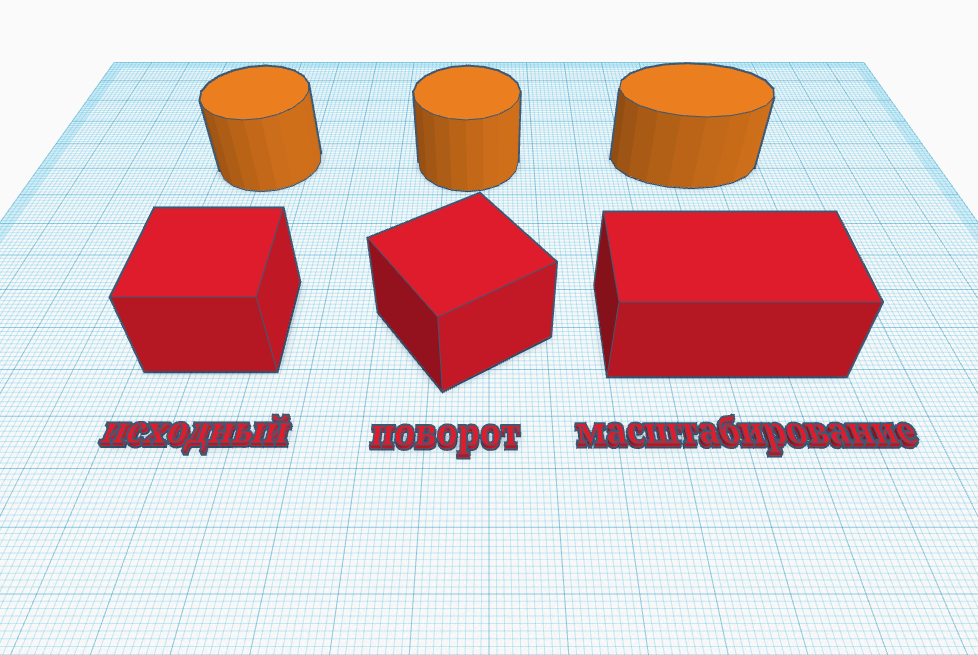
\includegraphics[scale=0.3]{inc/img/primitive_instancing}
  \caption{Пример клонирования примитивов на примере куба и цилиндра}
  \label{fig:primitive_instancing}
\end{figure}

\clearpage
Каждое семейство объектов называется общим примитивом, а отдельные объекты называются примитивными экземплярами.
Например, семейство болтов является общим примитивом, а отдельный болт, заданный определенным набором параметров (см. рис. \ref{fig:bolt}), является примитивным экземпляром.
\begin{figure}
  \centering
  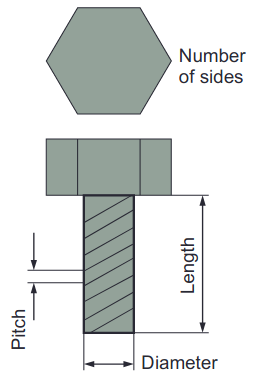
\includegraphics[scale=0.6]{inc/img/bolt}
  \caption{Болт задан параметрами: количество сторон головы, шаг резьбы, длина, диаметр}
  \label{fig:bolt}
\end{figure}

Особенности: 
\begin{itemize}
\item невозможно создать сложный объект, с помощью объединения экзепляров.
\end{itemize}

Минусы:  
\begin{itemize} 
\item cложность написания алгоритмов для вычисления свойств представленных твердых тел из - за уникальности каждого примитива, 
следовательно, обобщить обработку невозможно.
\end{itemize}

Плюсы:
\begin{itemize}
  \item способ хорош, если требуется только представление определённого семейства моделей.
\end{itemize}

Чтобы решить поставленную задачу, нужна схема, с помощью которой можно не зависеть от типа модели: его формы, параметров.

Рассмотрев схему можно заключить, что она не подходит для решения задачи, так как возникает потребность в подробном описании
всех свойств определённого семейства, а учитывая потребность в составных телах, сделать для них это будет проблематично.

\subsection{Нумерация пространственного заполнения} \label{numeric_scheme}
Cхема из себя представляет список-сетку пространственных ячеек, занятых твердым телом.
Ячейки (воксели) представляют собой кубы фиксированного размера (см. рис. \ref{fig:spatial_occupacy}) и расположены в заданной пространственной сетке. 
3D объект представляет собой список закрашенных вокселей.
\begin{figure}
  \centering
  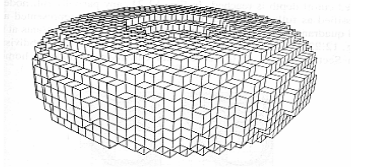
\includegraphics[scale=1.2]{inc/img/spatial_occupacy}
  \caption{Пример представления тора методом нумерации пространственного заполнения}
  \label{fig:spatial_occupacy}
\end{figure}

Каждая ячейка может быть представлена ​​координатами одной точки, например центроида ячейки.

Обычно устанавливается определенный порядок сканирования, и соответствующий упорядоченный набор координат называется пространственным массивом.

Пространственные массивы являются однозначными и уникальными твердыми представлениями, но слишком подробны для использования в качестве «основных» представлений \cite{lecture_solid_modeling}.

Минусы:  
\begin{itemize} 
\item затраты памяти высоки;
\item каждая ячейка хранит информацию о занятости, цвете, плотности и др.;
\item разрешение ограничено размером и формой вокселя.
\end{itemize}

Плюсы:
\begin{itemize}
  \item простая структура данных;
  \item однозначное представление.
\end{itemize}

Данная схема удобна с точки зрения простоты и точности представления, однако, структурно состоит из кубических форм,
для рендера, например, сферы, потребуется дополнительно сглаживать края, что накладывает дополнительную вычислительную нагрузку. 

Также для нас избыточно хранения в каждой ячейке информации о её состоянии.
Самостоятельное использование метода нецелесообразно, однако совместно с другими методами, можно использовать преимущество грубой апроксимации, для
повышения точности изображаемого тела. 
\subsection{Sweeping}
Эта схема позволяет создавать 3D модели из 2D с помощью движения по заданной траектории: вокруг оси (см. рис. \ref{fig:sweeping}), относительно граней и др. \cite{lecture_solid_modeling}.


\begin{figure}
  \centering
  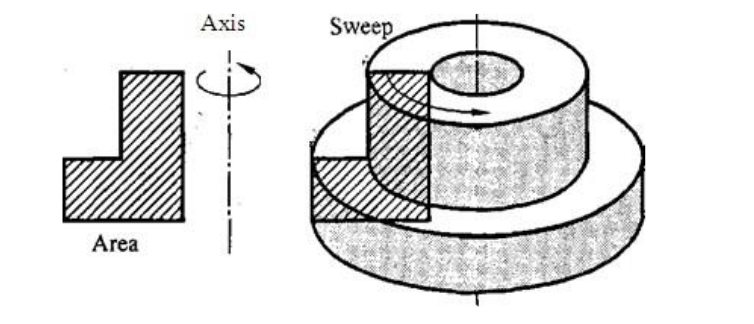
\includegraphics[scale=0.6]{inc/img/sweeping}
  \caption{Тело образовано вращением вокруг оси}
  \label{fig:sweeping}
\end{figure}

Плюсы:
\begin{itemize}
  \item простые формы удобно задавать через плоские фигуры;
  \item может использоваться для быстрого удаления материала внутри тела (см. рис. \ref{fig:sweeping_delete}).
\end{itemize}
\clearpage
\begin{figure}
  \centering
  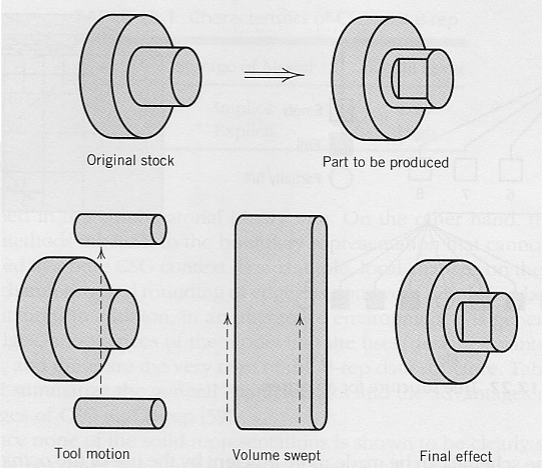
\includegraphics[scale=0.6]{inc/img/sweeping_delete}
  \caption{Удаление материала с помощью sweeping}
  \label{fig:sweeping_delete}
\end{figure}

Минусы:  
\begin{itemize}
\item необходимо задать траекторию движения 2D объекта, что проблематично для тел, имеющих сложную форму.
\end{itemize}
\subsection{Октантное дерево}
Схема является улучшением воксельного представления. Каждый узел октантного дерева соответствует некоторому кубу в трехмерном пространстве, для которого определяется принадлежность модели.
У каждого корня дерева есть 8 потомков, т.е куб делится на 8 равных частей (см. рис. \ref{fig:octree}).
\begin{figure}
  \centering
  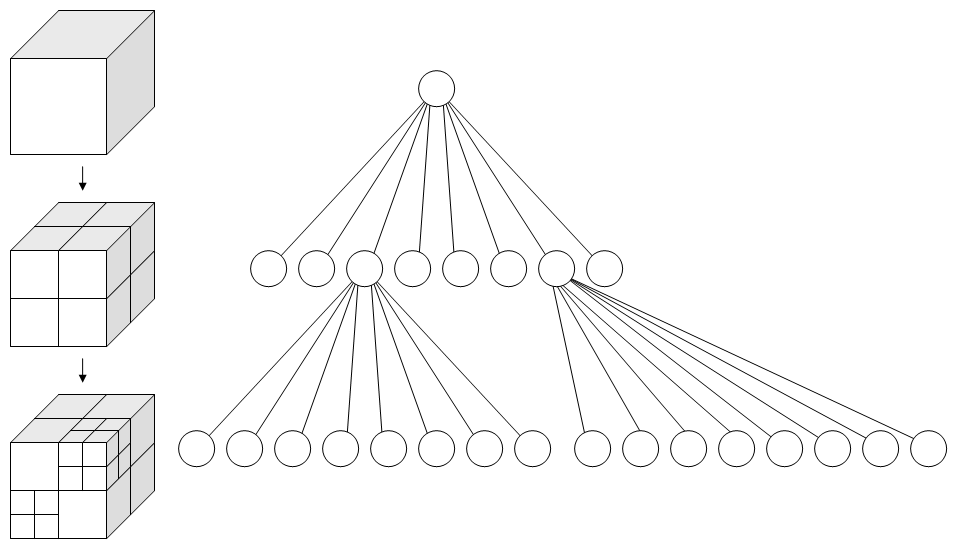
\includegraphics[scale=0.4]{inc/img/octree}
  \caption{Слева: Рекурсивное разделение куба на октанты. Справа: Соответствующее октодерево.}
  \label{fig:octree}
\end{figure}

Метод позволяет устранить недостаток метода \ref{numeric_scheme}, связанный с хранением большого количества данных, сохраняя информацию только об используемых частях модели.
Однако в сравнении с другими методами, памяти расходуется всё так же много. 

Обычно, используется в сферах, требующих точное представление, например, в медицине \cite{octree}.

Минусы:  
\begin{itemize} 
\item возможное деления примитива ребрами кубов дерева, что снижает эффективность;
\item вывод всех объектов, находящихся в поле камеры, но на самом деле в конечном счёте невидимых.
\end{itemize}

\subsection{Граничное представление(BREP)}
Способ представления модели с помощью границ. Замкнутая 2D-поверхность определяет 3D-объект.

Суть BRep-представления заключается в том, что твердое тело описывает замкнутая пространственная область,
ограниченная набором элементарных поверхностей (граней) с общими образующими  контурами (ребрами) на границе поверхностей (см. рис. \ref{fig:brep})
и признаком внешней или внутренней стороны поверхности.
\begin{figure}
  \centering
  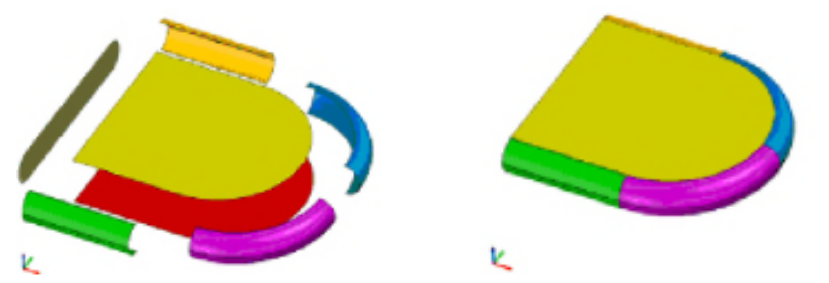
\includegraphics[scale=0.6]{inc/img/brep}
  \caption{BRep-представление простых твердых тел}
  \label{fig:brep}
\end{figure}

Данный способ проектирования в приложениях САПР является наиболее распространненным, 
однако имеет недостатки, из-за которых возникает проблема визуализации результата \cite{main_modeling}.


Минусы: 
\begin{itemize} 
\item высокие затраты памяти;
\item когда объект необходимо отрендерить объект требует слишком много вычислительной мощности;
\item для сложных объектов возникают трудности получения математических формул их описывающих.  
\end{itemize}

Плюсы:
\begin{itemize}
  \item подходит не только для твердых тел с плоскими гранями, но и для криволинейных объектов с замкнутыми криволинейными гранями или краями.
  \item позволяет проводить различные вычисления, требующие точность, благодаря хранению информации о всех составляющих модели.
\end{itemize}

\subsection{Конструктивная сплошная геометрия(CSG)}\label{csg}
Данный способ представления основан комбинирования примитивов посредством логических операций,
что позволяет создавать сложные модели на основе простых с помощью:
\begin{itemize}
  \item объединения;
  \item пересечения;
  \item разности.
\end{itemize}

Любое составное тело может быть описано в виде традиционного уравнения из булевых функций,
в котором аргументами являются либо элементарные тела, либо другие составные тела.
Это представление называют деревом построений (см. рис. \ref{fig:csg_tree}) \cite{main_modeling}.
\clearpage
\begin{figure}
  \centering
  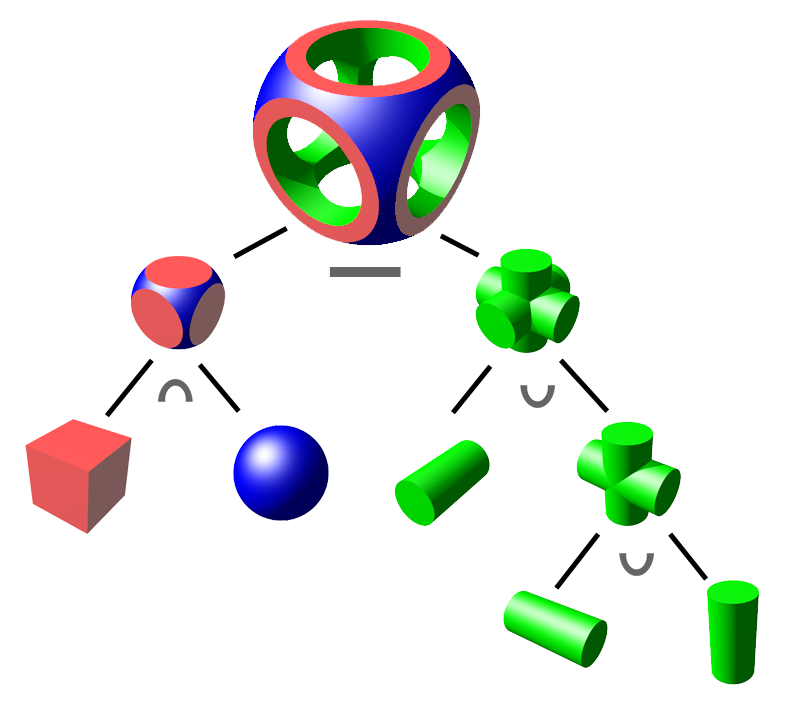
\includegraphics[scale=0.3]{inc/img/csg_tree}
  \caption{Сложный объект может быть представлен двоичным деревом, 
  где «листья» — это объекты, а узлы — операции. 
  ( пересечение, объединение, −  - разность)}
  \label{fig:csg_tree}
\end{figure}

Особенности:  
\begin{itemize}
  \item При использовании логических операций нужно иметь ввиду, что комбинирование может привести к вырождению твердого тела в плоское. 
\end{itemize}
\subsection{Сравнение схем}
Сравнивая схемы, предлагается разобрать следующие критерии:
\begin{enumerate}
  \item Лаконичность, т.е сколько памяти компьютера занимает модель (+ значит мало, - иначе: модель хранит не всегда используемую информацию), для решения задачи требуется минимальный расход;
  \item Эффективность, т.е насколько много времени необходимо для создания, исследования или изменения формы модели;
  \item Уникальность, т.е получить модель можно только одним способом;
  \item Однозначность, т.е вместе с моделью хранятся данные, которых достаточно для осуществления геометрических расчётов;
  \item Хранение истории преобразования модели, чтобы у пользователя была возможность вернуться к предыдущему шагу моделирования тела без применения афинных преобразований и дополнительных вычислений;
  \item Практичность, т.е создание модели без введения дополнительных параметров, поддерживая удобство использования.
\end{enumerate}
Разбор рассмотренных по критериям методов представлен в таблице 1.1.
\begin{table}[ht]
  \small
  \caption{Сравнительная таблица схем представления твёрдого тела}
  \begin{tabular}{|r|c|c|c|c|c|c|l|}
  \hline
  Методы&Лак-ть&Эф-ть&Ун-ть&Одноз-ть&История&Прак-ть\\
  \hline
  Клонирование примитивов  &-&+&-&+&-&-\\
  Нумер-я простр-го заполн. &-&-&+&+&-&-\\
  Октантное дерево & +& -& + & + & - & -\\
  BREP & -  & + & + & + & - & -\\
  Sweeping  & +  & - & - & + & -& -\\
  CSG  & + & + & - & + & + & + \\
  \hline
  \end{tabular}
  \label{tab:schemes}
\end{table}

После рассмотрения схем представления предлагается использовать CSG как наиболее подходящий метод создания моделей.
Представление  твердых  тел  в  виде  дерева  построений (листья - примитивы, узлы - результат операции) удобно также с точки зрения 
модификации объекта и организации пользовательского интерфейса, обеспечивающего наглядный и быстрый доступ к любому  элементу,
входящему  в  описание  геометрии тела. Остальные схемы требуют дополнительную информацию, которая необходима для обработки и создания моделей, 
но для решения задачи она не является необходимостью.


\clearpage


\section{Анализ методов рендера модели}
После того, как был выбран способ создания твердотельной модели, следует изучить методы рендера.  

Рендеринг (англ. rendering — «визуализация») "--- термин, обозначающий процесс получения изображения по модели с помощью компьютерной программы \cite{article:rendering}.\\
Рассмотрим возможные варианты:

\subsection{Растеризация}
Растеризация "--- это процесс получения растрового изображения \cite{article:rasterization}.\\
Растровое изображение - это изображение, представляющее собой сетку пикселей — цветных точек (обычно прямоугольных) на мониторе, 
бумаге и других отображающих устройствах \cite{article:rastr_image}.\\  
Технология основана на обходе лучем вершин треугольника (см. рис. \ref{fig:raster_scene}), 
который остаётся самим собой даже после попадания из трехмерного пространства в двухмерное.\\
\begin{figure}
  \centering
  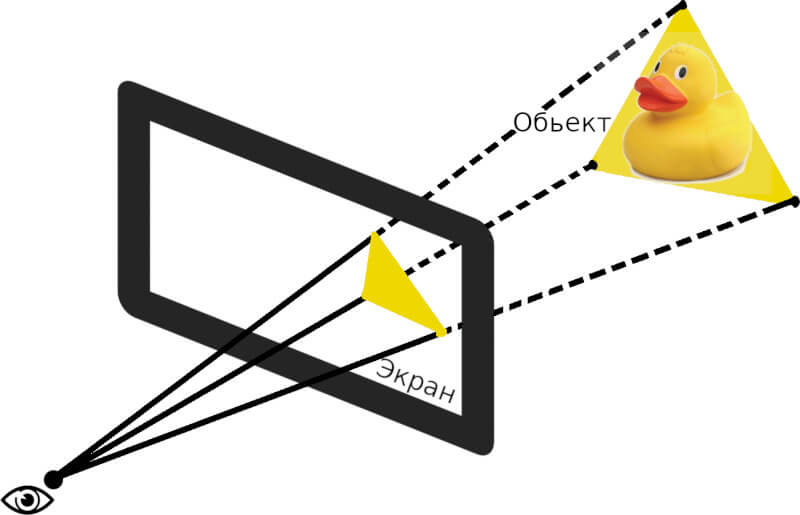
\includegraphics[scale=0.4]{inc/img/raster_scene}
  \caption{Схематическое отображение предмета на экран}
  \label{fig:raster_scene}
\end{figure}

\clearpage
Каждая точка каждого объекта в трехмерном пространстве переводится в точку на экране (см. рис. \ref{fig:raster_projection}),
а затем точки — заданные в модели треугольники — соединяются и получается изображение исходного объекта.\\

\begin{figure}
  \centering
  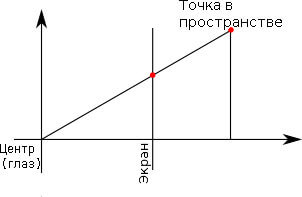
\includegraphics[scale=0.8]{inc/img/raster_projection}
  \caption{Проецирование точки из пространства на плоскость экрана, вид сбоку}
  \label{fig:raster_projection}
\end{figure}

Преимущества и недостатки:
\begin{itemize}
  \item изображение может быть "угловатым"(ступенчатым) - нуждается в сглаживании;
  \item требует больших вычислительных ресурсов - могут использоваться миллионы полигонов для всех моделей объектов сцены и примерно 8 миллионов пикселей на дисплее 4K,
  и каждый кадр или изображение, отображаемое на экране, обычно обновляется на дисплее от 30 до 90 раз в секунду \cite{nvidia:rastr};
  \item каждый пиксель обрабатывается много раз;
  \item 3D модель должна быть описана из примитивов, следовательно, составные модели обрабатывать ресурсозатратно, т.к нужно разбить его на примитивы, обычно, треугольники.
  \item современные компьютеры оптимизированы для рендеринга растровых изображений, благодаря чему этот процесс достаточно быстрый, однако, 
  как было сказано выше, с ростом сложности изображения, возрастают время рендера и потребности к ресурсам.
\end{itemize}
\clearpage

\subsection{Трассировка лучей}
\subsubsection{RayCasting}
Ray-casting (рус. — бросание лучей) "--- это технология, которая преобразует набор данных в 3D проекцию путем «бросания лучей» из точки обзора по всей области видимости. 

Основная идея -  испускать лучи из «глаз» наблюдателя, один луч на пиксель, и находить самый близкий объект,
который блокирует путь распространения этого луча (см. рис. \ref{fig:raycast_ex}). 
Последующая обработка преломленных от объекта лучей в этом методе отсутствует.
Используя свойства материала и эффект света в сцене, алгоритм бросания лучей может определить затенение данного объекта \cite{article:raycasting}.

\begin{figure}
  \centering
  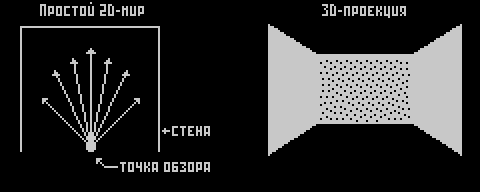
\includegraphics[scale=0.8]{inc/img/raycast_ex}
  \caption{На рисунке показано, как бросание преобразует что-то двумерное во что-то почти что трехмерное.}
  \label{fig:raycast_ex}
\end{figure}

Метод использовался при создании игр в конце прошлого века, такую графику иногда называют "псевдо 3D" или "2.5D". 

Из простоты алгоритма вытекает ряд ограничений, сказывающихся на качестве результата (см. рис. \ref{fig:raycast_game}), ведь на деле это
всего лишь трёхмерная проекция плоского изображения.
Ограничения алгоритма на примере применения в игровом мире \cite{article:who_to_work_raytrace}: 
\begin{enumerate}
  \item все доступное в игре пространство — это комната с прямоугольными (чаще квадратными) стенами;
  \item нет лестниц, лифтов, любого вида спусков и подъемов;
  \item потолок везде имеет одинаковую высоту;
  \item нет других трехмерных объектов, кроме стен, пола и потолка, все остальные объекты - двумерные изображения, расположенные в трехмерном пространстве.
\end{enumerate}
% На рисунке \ref{fig:raycast_game} изображена сцена из компьютерной игры $90$-х годов $XX$ века, демонстрирующая графические возможности алгоритма. 
\begin{figure}
  \centering
  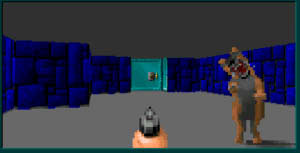
\includegraphics[scale=1]{inc/img/raycast_game}
  \caption{Сцена из Wolfenstein 3D. Картинка делится на прямоугольные блоки. Объекты (оружие) и враги (собака) — это просто прозрачные растровые изображения, которые масштабированы и отрисованы поверх заднего фона.}
  \label{fig:raycast_game}
\end{figure}

Минусы:
\begin{itemize}
  \item в результате рендера получается изображение среднего-плохого качества, в сравнении с остальным методами;
  \item геометрические ограничение на обрабатываемую поверхность(только простые фигуры);
  \item эффективен для объектов, у которых нет больших затрат на вычисление пересечения луча.
\end{itemize}

Плюсы:  
\begin{itemize}
  \item прост в реализации;
  \item нетребователен;
  \item изображение генерируется "на лету".
\end{itemize}
\subsubsection{RayTracing}
Трассировка лучей (англ. Ray Tracing) "--- это технология отрисовки трехмерной графики, симулирующая физическое поведение света \cite{article:who_to_work_raytrace}.\\
Принцип работы трассировки лучей:\\
поскольку все существующие трехмерные модели собраны из треугольников, 
нужно было обязательно сохранить обратную совместимость - для этого проверяется случай столкновения луча не со стеной, а с треугольником.
Рассмотрим его.
\begin{eqndesc}
Пусть вершины треугольника обозначены через $V_0$, $V_1$, $V_2$.
Векторы двух его рёбер обозначены как $A$, $B$ и заданы формулами \ref{eq:vector_triangle_a} и \ref{eq:vector_triangle_b}:\\
\begin{equation} \label{eq:vector_triangle_a}
  A = V_1 - V_0
\end{equation}
\begin{equation} \label{eq:vector_triangle_b}
  B = V_2 - V_0
\end{equation}
Определим луч $P$ с помощью параметрической формы уравнения \ref{eq:param_line}:
\begin{equation} \label{eq:param_line}
  P = R_0 + t \cdot R_d
\end{equation}
где $R_0$ "--- начальная точка луча, $R_d$ "--- направление луча, $t$ "--- расстояние вдоль луча, на которое попала точка\\
С другой стороны, точка пересечения имеет координаты $u$, $v$ в плоскости треугольника. Приравняв
уравнение луча $P$ и плоскости в точке $u$, $v$ (см. формулу \ref{eq:point_in_triangle}), можно найти пересечение:\\
\begin{equation} \label{eq:point_in_triangle}
  P = V_0 + u \cdot A + v \cdot B
\end{equation} 
Таким образом, составив систему из трех уравнений \ref{eq:system_for_coords} для координат $x, y, z$ и решив её для $t, u, v$, необходимо 
проанализировать определитель. Если он ненулевой(луч не параллелен плоскости), а $t >= 0$ и $u, v, u + v$ лежат в диапазоне от $0\dots1$, 
то $P$ находится внутри треугольника и поиск столкновения завершается.
 \\
\end{eqndesc}
\clearpage
\begin{eqndesc}
\begin{equation} \label{eq:system_for_coords}
\begin{aligned}
\begin{cases}
  R_0.x + t \cdot R_d.x = V_0.x + u \cdot A.x + v \cdot B.x \\
  R_0.y + t \cdot R_d.y = V_0.y + u \cdot A.y + v \cdot B.y \\
  R_0.z + t \cdot R_d.z = V_0.z + u \cdot A.x + v \cdot B.z \\
\end{cases}
\end{aligned}
\end{equation}
\end{eqndesc}

Особенность же трассировки лучей состоит в том, что на одном треугольнике серия вычислений не заканчивается, 
ведь некоторые поверхности могут быть зеркальными или просто блестеть. 
В таком случае луч не останавливается, а отражается от этого треугольника и снова ищет себе цель до тех пор, пока не вернётся в начальную точку, 
или не превысит максимальное число отражений.
Вся сложность алгоритма позволяет получить качественное изображения, в сравнении с полученным в результате растеризации (см. рис. \ref{fig:raster_vs_tracer}).

  \begin{figure}
  \centering
  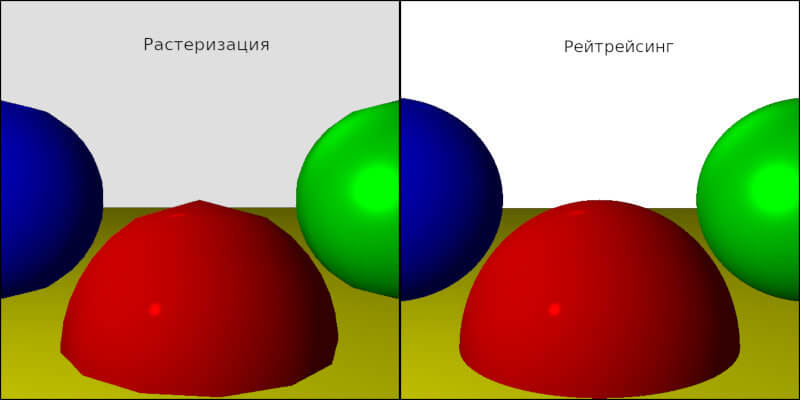
\includegraphics[scale=0.5]{inc/img/raster_vs_tracer}
  \caption{Сравнение растеризации и трассировки лучей}
  \label{fig:raster_vs_tracer}
\end{figure}
\clearpage

Плюсы: 
\begin{itemize}
  \item возможность рендеринга гладких объектов без аппроксимации их полигональными поверхностями (например, треугольниками);
  \item вычислительная сложность метода слабо зависит от сложности сцены;
  \item отсечение невидимых поверхностей, перспектива и корректное изменения поля зрения являются логическим следствием алгоритма.
\end{itemize}

Однако, главным недостатком метода является производительность. 
Метод трассирования лучей каждый раз начинает процесс определения цвета пикселя заново, 
рассматривая каждый луч наблюдения в отдельности. Что даёт изображению реалистичность, решает задачу отражения, но требует много ресурсов.\\
Следует рассмотреть модификацию данного алгоритма.  
\clearpage

\subsubsection{RayMarching}
Марширование лучей (англ. RayMarching) - разновидность алгоритма трассировки лучей.

Raymarching похож на традиционную трассировку лучей (raytracing) тем, что луч в сцену испускается для каждого пикселя. 
В трассировщике лучей есть набор уравнений, определяющих пересечение луча и рендерящихся объектов. 
Raymarching предлагает другой метод решения задачи пересечения луча и объекта, не пытается вычислить персечение аналитически.
При нём происходит смещение текущего положения вдоль луча, пока не будет найдена точка, пересекающая объект. 
Эта операция является относительно простой и малозатратной, гораздо более практичной в реальном времени.\\
Однако, этот способ не точно находит пересечение (см. рис. \ref{fig:raymarch_2}). 
\begin{figure}
  \centering
  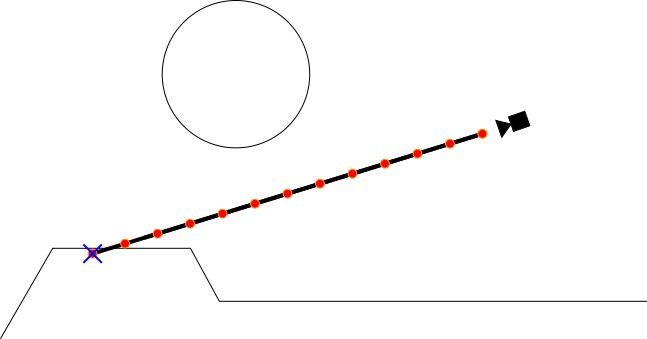
\includegraphics[scale=0.8]{inc/img/raymarch_2}
  \caption{Простейшая реализация метода с фиксированным интервалом шага. Красными точками обозначены все сэмплируемые точки.}
  \label{fig:raymarch_2}
\end{figure}

\subsubsection{Функция поля расстояний} \label{anl:sdf}
Реализация, разобранная выше, вполне достаточна для множества областей применения, например, объёмных и прозрачных поверхностей. 
Однако для непрозрачных объектов можно ввести ещё одну оптимизацию. 
Для этой оптимизации требуется использование полей расстояний со знаком. 

Поле расстояний (signed distance fields) "" --- это функция, получающая на входе точку и возвращающая кратчайшее расстояние от этой точки до поверхности каждого объекта в сцене. 
SDF возвращает отрицательное число, если точка находится внутри объекта. 

Этот инструмент позволяет нам ограничить количество шагов при движении вдоль луча (см. рис. \ref{fig:raymarch_3}),
что увеличивает эффективность метода.\\
\begin{figure}
  \centering
  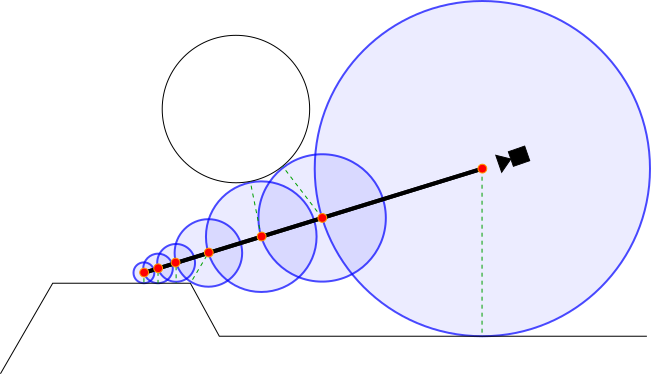
\includegraphics[scale=0.8]{inc/img/raymarch_3}
  \caption{Визуализация метода, с использованием SDF. Красными точками показаны все сэмплируемые точки. Синими кругами показаны области, которые гарантированно не содержат объектов (потому что они находятся в результатах функции поля расстояний). Пунктирными зелёными линиями показаны истинные кратчайшие векторы между каждой сэмплируемой точкой и сценой.}
  \label{fig:raymarch_3}
\end{figure}

Описание алгоритма \cite{article:who_to_work_3d}: 
\begin{itemize}
  \item для пикселя на экране определяется расстояние до ближайшего объекта;
  \item это расстояние определяет радиус на который можно пустить луч;
  \item пускаем луч;
  \item для конечной точки луча предыдущие пункты повторяются до тех пор пока следующий радиус не станет достаточно маленьким, 
  что будет означать столкновение с объектом. Или же радиус может начать стабильно увеличиваться, если луч прошел мимо всех объектов.
\end{itemize}
Плюсы:
\begin{itemize}
  \item решает проблему производительность трассировки лучей, работает быстро;
  \item подходит для рендера поверхностей, для которых сложно или невозможно вычислить пересечение аналитически;
  \item используя SDF можно ускорить рендеринг до реального времени;
  \item подходит для графического процессора, так как каждый пиксель можно рассчитать независимо;
  \item качество изображения сопоставимо с полученным при трассировке лучей.
\end{itemize}
Минусы:
\begin{itemize}
  \item пересечение вычисляется неточно, с некоторой погрешностью;
\end{itemize}
\clearpage
\subsubsection{Сравнение методов}
Сравнивая рассмотренные методы рендеринга, предлагается разобрать следующие критерии:
\begin{enumerate}
  \item качество;
  \item эффективность, т.е насколько много времени необходимо для рендера модели;
  \item выполнение в режиме реального времени;
  \item точность, т.е обработка истинных границ обрабатываемой модели;
\end{enumerate}
Разбор рассмотренных по критериям методов представлен в таблице \ref{tab:render}.
\begin{table}[ht]
  \caption{Сравнительная таблица методов рендеринга}
  \begin{tabular}{|r|c|c|c|c|}
  \hline
  Методы & Качество & Эффективность & Реал.время & Точность\\
  \hline
  Растеризация & - & + & + & + \\
  RayCasting & - & + & + & +\\
  RayTracing & + & - & - & +\\
  RayMarching & + & + & + & -\\
  \hline
  \end{tabular}
  \label{tab:render}
\end{table}

В данном разделе были рассмотрены методы рендера модели. Учитывая метод, выбранный в предыдущем  разделе, а также анализ в текущем,
можно сказать, что алгоритм raymarching наиболее привлекателен для рендера конструктивной сплошной геометрии,
в такой связке можно получить качественное изображение при его отрисовке в реальном времени. 
Один недостаток, это вычисление границ объекта с некоторой погрешностью, но остальные плюсы метода затмевают его.  
\section{Преобразования и визуализация}
В данном пункте рассматриваются средства для преобразования модели и 
придания ей трехмерного вида.
\subsection{Шейдеры}
Шейдер -  компьютерная программа, предназначенная для исполнения процессорами видеокарты (GPU) \cite{article:shaders}.

В разрабатываемом приложении использование шейдеров необходимо для придания изображению трехмерного вида, 
используя тени, освещение. 
Для этого предназначены фрагментный и вершинный шейдеры.
\subsubsection{Вершинные шейдеры} \label{anl:vert_shader}
Вершинный шейдер получает вершину из списка вершин и отображает ее в пространстве.
Вершинному шейдеру передаются следующие данные:
\begin{itemize}
  \item матрица модели;
  \item матрица вида;
  \item матрица проекции.
\end{itemize}

Матрица модели:

Необходима для перехода от пространства модели (все вершины определены относительно центра модели) 
в мировое пространство (все вершины определены относительно центра мира).

Матрица вида:

Необходима для перемещения сцены относительно камеры. В реальном мире происходит перенос самой камеры, точки обзора. 
В компьютерной графике более просто и удобно переместить сцену относительно камеры, тем самым в результате 
получить перемещение камеры относительно сцены.  

Матрица проекции:

Эта матрица используется для представления перспективы камеры. Умножение координат на данную матрицу 
позволяет сопоставить вершину с перспективой камеры, учитывая ее соотношения сторон, поля обзора
и самого дальнего и ближайшего объекта, который виден. 

Для преобразования координат выполняются следующие действия:
\begin{enumerate}
  \item положение вершины умножается на матрицу модели, чтобы определить, где эта вершина находится относительно центра модели в сцене;
  \item результат умножается на матрицу вида, чтобы определить, где расположена вершина относительно камеры;
  \item результат второй операции умножается на матрицу проекции, чтобы определить, где находится вершина в перспективе камеры. 
\end{enumerate}
\subsubsection{Фрагментные шейдеры}
Фрагментный шейдер работает с пикселями объекта и управляет цветом пикселя.
Выполнение фрагментного шейдера в графическом конвейере происходит после вершинного, следовательно, никак не влияет на координаты вершины,
он влияет только на цветовую составляющую, преобразуя вершины уже в пиксели или фрагменты.

Помимо придания трехмерного вида, к моделям следует применять операции, 
которые позволяют изменять их положение и ориентацию. 
\subsection{Матрицы преобразования}
Для преобразования тела в пространстве используются операции:
\begin{itemize}
  \item перемещения;
  \item масштабирования;
  \item поворота.
\end{itemize}

Осуществляются преобразования с помощью матриц \ref{tab:matrix}. 
\begin{table}[ht]
\small
\caption{Таблица преобразований}
\begin{tabular}{|l|c|l|}
\hline
Преобразование & Матрица & Формула\\
\hline
Перемещение      & $\begin{pmatrix}
    1  & 0  & 0  & 0 \\
    0  & 1  & 0  & 0 \\
    0  & 0  & 1  & 0 \\
    dx & dy & dz & 1
  \end{pmatrix}$  & $\begin{cases}
    x_1=x+dx \\
    y_1=y+dy \\
    z_1=z+dz
  \end{cases}$  \\
\hline
Масштаб - е  & $\begin{pmatrix}
    k_x & 0   & 0   & 0 \\
    0   & k_y & 0   & 0 \\
    0   & 0   & k_z & 0 \\
    0   & 0   & 0   & 1
  \end{pmatrix}$ & $\begin{cases}
    x_1=k_x+(1-k_x)x_m \\
    y_1=k_y+(1-k_y)y_m \\
    z_1=k_z+(1-k_z)z_m
  \end{cases}$ \\
\hline
Поворот OX & $\begin{pmatrix}
    1 & 0           & 0          & 0 \\
    0 & \cos\theta  & \sin\theta & 0 \\
    0 & -\sin\theta & \cos\theta & 0 \\
    0 & 0           & 0          & 1
  \end{pmatrix}$ & $\begin{cases}
    x_1=x                                       \\
    y_1=y_c+(y-y_c)\cos\theta-(z-z_c)\sin\theta \\
    z_1=z_c+(y-y_c)\sin\theta+(z-z_c)\cos\theta
  \end{cases}$ \\
\hline
Поворот OY & $\begin{pmatrix}
    \cos\theta & 0 & -\sin\theta & 0 \\
    0          & 1 & 0           & 0 \\\sin\theta&0&\cos\theta&0 \\
    0          & 0 & 0           & 1
  \end{pmatrix}$ & $\begin{cases}
  x_1=x_c+(x-x_c)\cos\theta+(z-z_c)\sin\theta \\
  y_1=y \\
  z_1=z_c-(x-x_c)\sin\theta+(z-z_c)\cos\theta
  \end{cases}$ \\
\hline
Поворот OZ & $\begin{pmatrix}
    \cos\theta  & \sin\theta & 0 & 0 \\
    -\sin\theta & \cos\theta & 0 & 0 \\
    0           & 0          & 1 & 0 \\
    0           & 0          & 0 & 1
  \end{pmatrix}$ & $\begin{cases}
    x_1=x_c+(x-x_c)\cos\theta-(y-y_c)\sin\theta \\
    y_1=y_c+(x-x_c)\sin\theta+(y-y_c)\cos\theta \\
    z_1=z
  \end{cases}$ \\
\hline
\end{tabular}
\label{tab:matrix}
\end{table}
\clearpage

Исходные координаты объекта умножаются на одну или несколько матриц, в результате чего
объект перемещается/масштабируется/поворачивается, в зависимости от примененных преобразований.  
Помимио этого, матрицы позволяют перевести координаты модели в мировые, переместить сцену относительно камеры, настроить перспективу.

В данном пункте были рассмтрены средства для преобразования модели - матрицы преобразования, а также
для преобразования плоского изображения в трехмерный вид - шейдеры.
\section{Аппаратная обработка}
В данном разделе предлагается рассмотреть аппаратную составляющую рендеринга.
Есть 2 основных варианта: рендеринг на центральном и графическом процессорах.
Они имеет много общего, но существуют различия,
которые оказывают огромное влияние на скорость и качество изображения. 
Рендеринг на базе ЦП является традиционным способом и широко используется. Напротив, рендеринг с помощью графических процессоров 
с годами становится все более популярным в сообществе благодаря быстроразвивающемуся миру технологий.
Рассмотрим подробнее каждый из процессоров.
\subsection{CPU}
CPU "--- центральный процессор, это основной компонент компьютера, обрабатывающий инструкции. 
Он выполняет вычисления, действия, запускает программы, включая рендеринг. 
Центральный процессор постоянно принимает ввод от пользователя или активных программ, затем обрабатывает данные и выдает вывод, который может быть сохранен приложением или отображен на экране \cite{article:cpu_gpu}.
\subsection{GPU}
GPU "--- графический процессор. Разработан для параллельной обработки трудоёмких вычислительных задач. 
Графический процессор используется в широком спектре приложений, ускоряющих рендеринг 3D-графики.
Кроме того, этот микропроцессор также используется для разгрузки некоторых задач с центрального процессора, что заставляет компьютер работать быстрее \cite{article:cpu_gpu}.
\subsection{Сравнение процессоров}
Рассмотрим различия процессоров приминительно к рендеру \cite{cpu_or_gpu}:
\begin{enumerate}
  \item главное различие между процессорами CPU и GPU заключается в том, как каждый из них выполняет разные задачи;
  \item архитектурно CPU состоит всего из нескольких ядер с большим количеством кэш-памяти, которая может обрабатывать несколько программных потоков одновременно, 
  Напротив, графический процессор состоит из сотен меньших и более эффективных ядер, которые могут одновременно выполнять несколько задач и быстрее обрабатывать изображения;
  \item рендеринг с помощью графического процессора более эффективен с точки зрения задач обработки, требующих нескольких параллельных процессов,
  фактически, рендеринг GPU примерно в 10-100 раз быстрее, чем рендеринг CPU;
  \item GPU позволяет в реальном времени просматривать и манипулировать 3D моделями, источниками света и проекциями в трех измерениях. Некоторое программное обеспечение для рендеринга, 
  предназначенное только для графического процессора, может даже позволить полностью работать в окне просмотра с включенным Real Time рендерингом, увеличивая результат и минимизируя возможные ошибки, которые могут возникнуть при рендеринге в другой программе. 
  CPU же не позволяет рендерить в реальном времени качественные изображения.
\end{enumerate}


Изначальная цель заключалась в создании приложения для рендера 3D модели в режиме реального времени.
Такой сценарий позволяет осуществить рендеринг на видеокарте, следовательно, для поставленной задачи следует выбрать её, а не CPU.  

\section{Вывод} \label{anl:algo_choice}
В данной главе был проведен анализ возможных методов для решения поставленной задачи. 
В качестве метода создания модели, при помощи которого будет решаться задача, была выбрана CSG,
рендера -- RayMarching. Для преобразования модели будут использоваться матрицы преобразований, для придания изображению
трехмерного вида - шейдеры. На GPU ложится графическая составляющая задачи, а на CPU -  взаимодействие с пользователем.


% %%% Local Variables:
% %%% mode: latex
% %%% TeX-master: "rpz"
% %%% End:

\chapter{Конструкторский раздел}
\label{cha:design}

В данном разделе рассматриваются реализуемые методы, алгоритмы. Приводится
схема приложения и диаграмма классов.

\section{Метод конструктивной сплошной геометрии}
Данный метод делится на несколько алгоритмов, рассматриваемых ниже.

% \subsection{Знаковая функция расстояния и алгоритмы композиции тел}
Знаковая функция расстояния (англ. $SDF$) может быть использована для получения кратчайшего 
расстояния от точки до поверхности тела, причём отрицательный знак соответствует положению точки внутри тела.
Ниже рассматриваются $SDF$ для сферы и куба.

Для получения $SDF$ сферы необходимо знать расстояние до её центра от заданной точки (см. формулу \ref{eq:center_of_sphere})
и длину радиуса.
\begin{equation} \label{eq:center_of_sphere}
  length(x,y,z) = \sqrt{(x - x_0)^2 + (y - y_0)^2 + (z - z_0)^2}
\end{equation}
где $C(x_0, y_0, z_0)$ - центр координат,
$p(x, y, z)$ - рассматриваемая точка.  

Подставляя формулу \ref{eq:center_of_sphere} в формулу расстояния \ref{eq:sdf_sphere} можно получить
$SDF$ сферы.
\begin{equation} \label{eq:sdf_sphere}
  dist = length(x, y, z) - r
\end{equation}
Для куба необходимо учесть 3 расположения точки относительно граней и 
получить формулу \ref{eq:sdf_box} $SDF$ куба.
% объединить всё в одну формулу (см. \ref{eq:sdf_box}), получив SDF куба.
\begin{equation} \label{eq:sdf_box}
  \begin{cases}
    q = abs(p) - r  \\
    dist = length(max(q, 0.0)) + min(max(q.x, max(q.y,q.z)), 0.0)
  \end{cases}
\end{equation}
где $p(x, y, z)$ - рассматриваемая точка,
$q(x, y, z)$ - координаты точки за вычетом радиуса,
$dist$ - искомое расстояние с учётом двух расположений точки относительно граней и угла.

Данные $SDF$ позволяют эффективно использовать алгоритм маршировки лучей, так как луч двигается
к рассматриваемому объекту с максимальным шагом, который не приведёт к пропуску лицевой грани объекта.

$SDF$ используется в моделировании тел $CSG$.
Алгоритмы композиции необходимо использовать, чтобы связать методы создания тел и визуализации

При пересечении двух тел (см. формулу \ref{eq:sdf_intersect}) луч должен пересечься с тем, которое дальше от камеры, следовательно,
необходимо выбрать $SDF$ с наибольшим значением.
\begin{equation} \label{eq:sdf_intersect}
  intersection(sdf1, sdf2, x, y, z) = max(sdf1(x, y, z), sdf2(x, y, z))
\end{equation}
где $sdf1$, $sdf2$ - функции, возвращающие расстояние до точки с координатами $x$, $y$, $z$.

Для объединения (см. формулу \ref{eq:sdf_union}) тел луч должен пересечься с ближайшим телом, следовательно, 
нужно выбрать $SDF$ с минимальным значением.
\begin{equation} \label{eq:sdf_union}
  union(sdf1, sdf2, x, y, z) = min(sdf1(x, y, z), sdf2(x, y, z))
\end{equation}

В методе $CSG$ имеет важность порядок параметров при поиске разности, которая является некоммутативной операцией.
Необходимо определить порядок тел - операндов и найти максимальной расстояние между первым и вторым телом.
Расстояние до второго тела берётся с отрицательным знаком.
Луч должен пересечься с первым телом и не пересечься с вторым, следовательно, второе тело
можно представить в виде всего пространства за пределами второго тела (см. формулу \ref{eq:invert_union}) с помощью
инвертирования. 
\begin{equation} \label{eq:invert_union}
  invert(sdf, x, y, z) = -sdf(x, y, z)
\end{equation}

Теперь можно найти пересечние (см. формулу \ref{eq:sdf_diff}) первого тела и инвертированного второго:
\begin{multline} \label{eq:sdf_diff}
  diff(sdf1, sdf2, x, y, z) = union(sdf1(x, y, z), invert(sdf2, x, y, z)) =\\
  min(sdf1(x, y, z), -sdf2(x, y, z)))
\end{multline}

\section{Алгоритм raymarching}\label{alg:raymarch}
Выбранный алгоритм raymarching отрисовывает объекты с помощью $SDF$.
Маршировка лучей предполагает иттеративное перемещение точки вдоль луча обзора (от камеры к объекту) и проверку
результата: отрицательный знак возвращенного значения показывает столкновение с объектом. 

$Raymarching$ использует границы сцены,
которые должны передаваться в качестве входных данных алгоритму.
Алгоритм $raymarching$ представлен на псевдокоде \ref{psevdo:raymarch}.
\begin{algorithm}
\caption{Алгоритм маршировки лучей}\label{psevdo:raymarch}
\begin{algorithmic}[1]
  \Function{rayMarch}{start, end}
  \State $depth$ $\leftarrow$ $start$
  \State $i$ $\leftarrow$ $0$
  \While {$i < MAX\_STEPS$}
    \State $dist$ $\leftarrow$ расстояние до объекта
    \If {внутри объекта}
      \State \Return $depth$
    \EndIf
    \State $depth += dist$
    \State $i += 1$
    \If {луч вышел за пределы сцены}
      \State \Return $end$
    \EndIf
  \EndWhile
  \State \Return $end$
  \EndFunction
\end{algorithmic}
\end{algorithm}
\clearpage
% \begin{lstlisting}[language=GLSL, label=lst:raymarch, caption = {Реализация алгоритма нахождения raymarching}]
%   /*
%  * Функция возвращает кратчайшее расстояние от начальной точки до поверхности сцены вдоль направления движения луча.
%  * Если между началом и концом не найдено поверхности, возвращает конец.
%  * 
%  * eye: точка обзора, являющаяся источником луча
%  * marchingDirection: нормализованное направление луча
%  * start: начальная точка движения луча
%  * end: максимальное расстояние от начала к концу, делающее алгоритм конечным
%  *
%  * sceneSDF - знаковая функция расстояния, описывающая сцену. 
%  * Абсолютное значение возвращаемого значения указывает расстояние до поверхности.
%  * Знак указывает, находится ли точка внутри или за пределами поверхности:
%  * "+" - точка вне поверхности,
%  * "-" - точка внутри поверхности.
%  */
%   float shortestDistanceToSurface(vec3 eye, vec3 marchingDirection, float start, float end) {
%     float depth = start;
%     for (int i = 0; i < MAX_MARCHING_STEPS; i++) {
%         float dist = sceneSDF(eye + depth * marchingDirection);
%         if (dist < EPSILON) {return depth;}
%         depth += dist;
%         if (depth >= end) {return end;}
%     }
%     return end;
% }
% \end{lstlisting}
% \subsection{Алгоритмы композиции тел} \label{alg:sdf}
% $CSG$ построен на трех примитивных операциях: пересечение, объединение, разность.
% Чтобы связать методы создания тел и визуализации, необходимо использовать алгоритмы композиции тел, 
% рассмотренные ниже.

% При пересечении двух тел луч должен пересечься с тем, которое дальше от камеры, следовательно,
% необходимо выбрать $SDF$ с наибольшим значением \ref{eq:sdf_intersect}.

% \begin{equation} \label{eq:sdf_intersect}
%   intersection(csg1, csg2, x, y, z) = max(csg1(x, y, z), csg2(x, y, z))
% \end{equation}
% где $csg1$, $csg2$ - функции, возвращающие расстояние до точки с координатами $x$, $y$, $z$.

% % Для поиска пересечения необходимо найти максимальное расстояние до объектов в данной точке,
% % так как необходимо найти области тела, которые относятся к обоим объектам.

% % Для объединения необходимо найти минимальное расстояние (области, относящиеся либо к первому телу, либо
% % ко второму).
% Для объединения тел луч должен пересечься с ближайшим телом, следовательно, 
% нужно выбрать $SDF$ с минимальным значением \ref{eq:sdf_union}.

% \begin{equation} \label{eq:sdf_union}
%   union(csg1, csg2, x, y, z) = min(csg1(x, y, z), csg2(x, y, z))
% \end{equation}

% В методе $CSG$ имеет важность порядок параметров при поиске разности, которая является некоммутативной операцией.
% Необходимо определить порядок тел - операндов и найти максимальной расстояние между первым и вторым телом.
% Расстояние до второго тела берётся с отрицательным знаком.
% Луч должен пересечься с первым телом и не пересечься с вторым, следовательно, второе тело
% можно представить в виде всего пространства за пределами второго тела. 
% Запишем функцию инвертирования: 

% \begin{equation} \label{eq:invert_union}
%   invert(csg, x, y, z) = -csg(x, y, z)
% \end{equation}
  
% Теперь задача решается с помощью пересечения первого тела и инвертированного второго:
% \begin{multline} \label{eq:sdf_diff}
%   diff(csg1, csg2, x, y, z) = union(csg1(x, y, z), invert(csg2, x, y, z)) =\\
%   min(csg1(x, y, z), -csg2(x, y, z)))
% \end{multline}

% % Алгоритмы реализации приведены на листинге \ref{lst:body_compose}
% % \begin{lstlisting}[language=GLSL, label=lst:body_compose, caption = {Реализация алгоритмов композиции тел}]
% %  /*
% %  * Операция пересечения 
% %  * distA, distB: расстояние до объектов
% %  *
% %  * Функция возвращает максимальное расстояние из двух
% %  */
% %   float intersectSDF(float distA, float distB) {
% %     return max(distA, distB);
% % }
% % /*
% % * Операция объединения 
% % * distA, distB: расстояние до объектов
% % *
% % * Функция возвращает минимальное расстояние из двух
% % */
% % float unionSDF(float distA, float distB) {
% %     return min(distA, distB);
% % }
% % /*
% % * Операция разности 
% % * distA, distB: расстояние до объектов
% % *
% % * Функция возвращает максимальное расстояние из двух.
% % */
% % float differenceSDF(float distA, float distB) {
% %     return max(distA, -distB);
% % }
% % \end{lstlisting}
% % Следует рассмотреть подробнее операцию разности, а именно, почему второй параметр взят с противоположным знаком.

% % В SDF отрицательный знак означает внутреннюю поверхность объекта. 
% % Таким образом, инвертируя второй параметр, позволяет изменить анализируемую часть модели: 
% % внутренняя поверхность становится внешней и наоборот.  

% % В результате, SDF сцены будет отрицательным, и следовательно луч достигнет сцены, только тогда, 
% % когда первый SDF отрицательный, а второй положительный.  

\section{Схема приложения}
В данном пункте приведена схема частей приложения, а также подробно рассмотрено моделирование тела.

Всё приложение строится из частей, приведённых на рисунке \ref{fig:app_scheme}.

\begin{figure}[H]
  \centering
  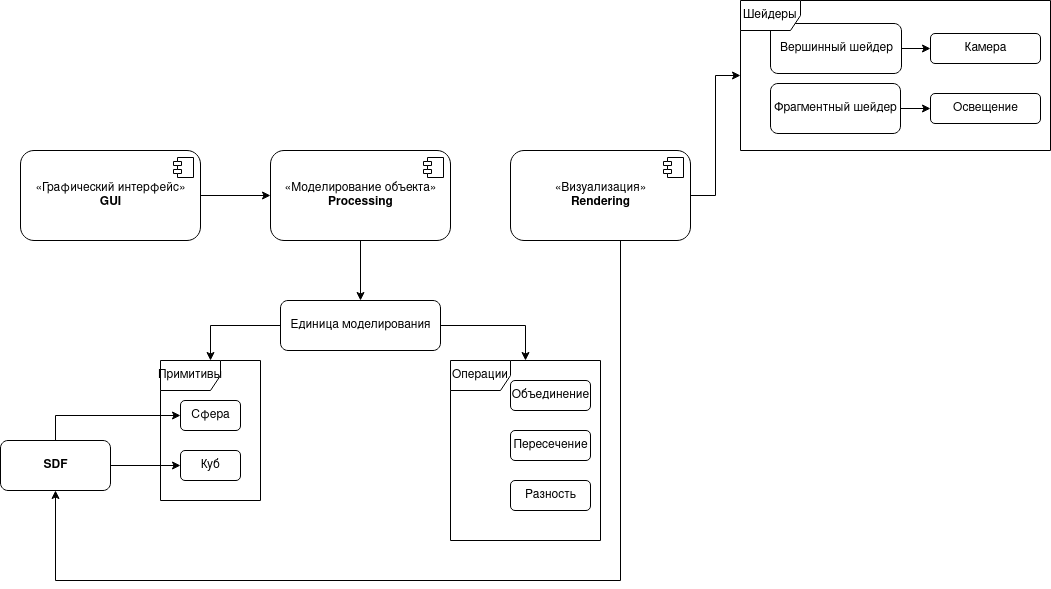
\includegraphics[scale=0.4]{inc/img/component_diagram}
  \caption{Схема приложения}
  \label{fig:app_scheme}
\end{figure}

На схеме представлено приложение, разделенное на функциональные части.
Пользователь может задать входные данные в графическом интерфейсе ($GUI$): примитивы, типы операций над ними,
положение камеры.
Выполнение отрисовки требует предварительного моделирования тела ($Processing$), которое описано рисунком \ref{fig:classes_diagram}, после
которого следует этап отрисовки, использующий шейдеры для установки положения камеры и выставления теней ($Rendering$).
% С помощью шейдеров модель закрашивается с учётом освещения.
% В результате полученное изображения отображается на экране и пользователь имеет возможность менять положение камеры.
% Весь процесс продолжается, пока пользователь не завершит выполнение.
% Для этапа моделирования были разработаны классы, которые представлены на рисунке \ref{fig:classes_diagram}.
% Помимо схемы, для проектируемого ПО приводится диаграмма классов моделирования тела ($Processing$ на схеме приложения).
% 
% \begin{figure}[H]
  % \centering
  % 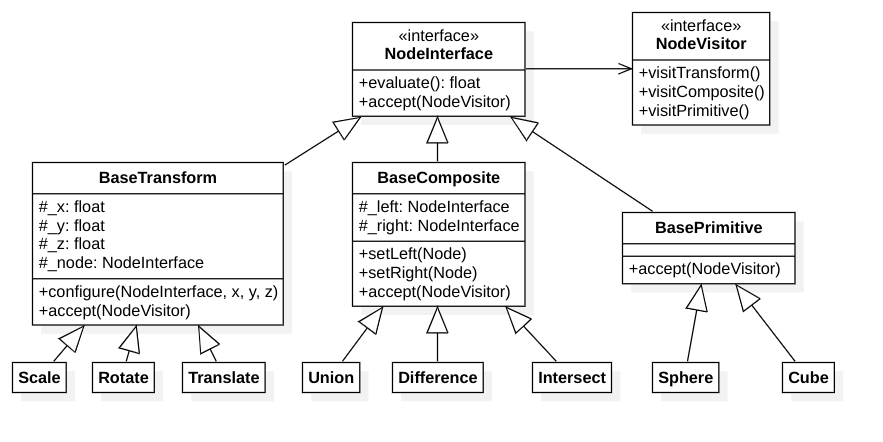
\includegraphics[scale=0.35]{inc/img/classes_diagram}
  % \caption{Диаграмма классов Processing}
  % \label{fig:classes_diagram}
% \end{figure}

% Для создания объектов в $CSG$ используется двоичное дерево.
% Данное дерево состоит из узлов, которые представлены в виде классов $Node$, которые являются реализацией интерфейса - 
% $BaseTransform$, $BaseComposite$, $BasePrimitive$.
% Класс $NodeInterface$ задаёт интерфейс для операций преобразования тел. 
% Все операции над моделью разделены на три группы: операции преобразования,
% операции композиции, операции создания примитивов. 

% Класс $BaseTransform$ предназначен для преобразования тела. Он содержит координаты 
% для перемещения/масштабирования/поворота модели. 
% Метод $configure$ конструирует экземпляр класса, принимая на вход модель - узел и координаты.  
% Класс $BaseComposite$ предназначен для конструирования модели с помощью $CSG$.  
% Он представляет собой дерево. Результатом обхода является модель. 
% Класс $BasePrimitive$ предназначен для создания примитивов, из которых происходит построение 
% модели.
% Класс $NodeVisitor$ реализует паттерн проектирования "Посетитель" и необходим для добавления
% нового функционала классам. В разрабатываемом ПО этот паттерн позволяет определить,
% какой класс представлен в $NodeInterface$, т.к его использование интерфейса подразумевает 
% абстрагирование от наследуемых реализаций. Обход происходит с помощью методов 
% $visitTransform$, $visitComposite$, $visitPrimitive$.  


\section{Вывод}
В данном разделе были рассмотренны методы и алгоритмы, необходимые для создания 
приложения. Была приведена схема приложения, представляющая архитектура проектируемого приложения.


%%% Local Variables:
%%% mode: latex
%%% TeX-master: "rpz"
%%% End:

\chapter{Технологический раздел}
\label{cha:impl}
В данном разделе представленны средства разработки программного обеспечения, детали реализации и тестирование функций.
\section{Средства реализации}
В качестве языка программирования, на котором будет реализовано программное обеспечение, выбран язык программирования JavaScript \cite{impl:js}. Выбор языка обусловлен тем, что данный язык является языком программирования для бразуера,
что позволяет запускать приложение в браузере и делает его кроссплатформенным решением, а также позволяет запускать приложение без установки дополнительных зависимостей. Помимо этого, для JavaScript существует бибиотека 
ThreeJS \cite{impl:three_js}, которая предоставляет canvas (холст), на котором происходит отрисовка сцены, модуль для работы с камерой, а также позволяет подключить шейдеры, используя небольшое количество подготовительных этапов.
Для создания пользовательского интерфейса программного обеспечения будет использоваться модуль dat-gui \cite{impl:dat_gui}. Этот модуль позволяет предоставить пользователю возможность изменять параметры модели.
Для мониторинга производительности будет использоваться модуль Stats \cite{impl:stats_js}. Этот модуль позволяет отслеживать FPS (количество кадров в секунду). Данная информация поволит оценить производительность ПО.
Функциональное тестирование ПО проводиться не будет из-за своей специфики -- разработанное ПО является GUI-приложением, что усложняет процесс тестирования.
В качестве среды разработки выбран текстовый редактор Visual Studio Code \cite{impl:vscode}, содержащий большое количеством плагинов и инструментов для различных языков программирования, в том числе JavaScript. Такие инструменты облегчают и ускоряют процесс разработки программного обеспеченияd.
Для запуска приложения используется python сервер \cite{impl:python}, позволяющий использовать ПО в браузере.  
\section{Детали реализации}
В листингах \ref{lst:body_compose} -- \ref{lst:raymarch} приведен исходный код реализации алгоритмов
для преобразования тел и отрисовки на сцене модели.
Алгоритмы отрисовки модели были разделены на подпрограммы:  
получение расстояния до каждого из объектов (куб, цилиндр, сфера), получение расстояния до композии объектов,
пускание луча.
\begin{lstlisting}[language=GLSL, label=lst:body_compose, caption = {Реализация алгоритмов композиции тел}]
 /*
 * Операция пересечения 
 * distA, distB: расстояние до объектов
 *
 * Функция возвращает максимальное расстояние из двух
 */
 float intersect(float distA, float distB) {
  return max(distA, distB);
}
/*
* Операция объединения 
* distA, distB: расстояние до объектов
*
* Функция возвращает минимальное расстояние из двух
*/
float union(float distA, float distB) {
  return min(distA, distB);
}
/*
* Операция разности 
* distA, distB: расстояние до объектов
*
* Функция возвращает максимальное расстояние из двух.
*/
float difference(float distA, float distB) {
  return max(distA, -distB);
}
\end{lstlisting}
\newpage
\begin{lstlisting}[language=GLSL, label=lst:transform, caption = {Реализация алгоритмов преобразования тела}]
/*
* Операция переноса
*/
vec3 translate(vec3 p, vec3 v) {
  return p - v;
}
/*
* Операция поворота
*/
vec3 rotate(vec3 p, vec3 rad) {
  float x, y, z = rad.x, rad.y, rad.z;
  mat3 m = mat3(
    cos(y)*cos(z),
    sin(x)*sin(y)*cos(z) - cos(x)*sin(z),
    cos(x)*sin(y)*cos(z) + sin(x)*sin(z),

    cos(y)*sin(z),
    sin(x)*sin(y)*sin(z) + cos(x)*cos(z),
    cos(x)*sin(y)*sin(z) - sin(x)*cos(z),

    -sin(y),
    sin(x)*cos(y),
    cos(x)*cos(y)
  );
  return m * p;
}
\end{lstlisting}
\begin{lstlisting}[language=GLSL, label=lst:raymarch, caption = {Реализация алгоритмов пускания луча для отрисовки поверхностей}]
/*
* Функция пускания луча
*/
float getDistance(vec3 rayOrigin, vec3 rayDirection, out vec3 rayPosition, out vec3 normal, out bool hit) {
    float dist, depth = 0.0, 0.0;
    rayPosition = rayOrigin;

    for (int i = 0; i < 64; i++){
        dist = sceneDist(rayPosition);
        if (abs(dist) < EPS) {
            hit = true;
            break;
        }
        depth += dist;
        rayPosition = rayOrigin + depth * rayDirection;
    }
    return depth;
}
/*
* Функция получения расстояния до объекта
*/
float sceneDist(vec3 p) {
  return distance(p);
}
/*
* Функция получения расстояния до конкретной сцены - разность объединения куба и цилиндра с сферой
*/
float distance(vec3 p) {
  float cube = boxDist(rotate(translate(p, cubePosition), cubeRotation), vec3(cubeScale * 2., cubeScale * 2., cubeScale * 2.));
  float cylinder = cylinderDist(rotate(translate(p, cylinderPosition), cylinderRotation), cylinderScale * 0.5, cylinderScale * 4.0);
  float sphere = sphereDist(translate(p, spherePosition), sphereScale * 1.);

  return difference(union(cube, cylinder), sphere);
}
\end{lstlisting}
\section{Вывод}
В данном разделе были рассмотренны средства реализации программ-
ного обеспечения и листинги исходных кодов программного обеспечения,
разработанного на основе алгоритмов, изученных в аналитическом разделе и изложенных в 
конструкторской части.
%%% mode: latex
%%% TeX-master: "rpz"
%%% End:

% \chapter{Экспериментальный раздел}
\label{cha:research}

В данном разделе проводятся вычислительные эксперименты.
А на рис.~\ref{fig:spire01} показана схема мыслительного процесса автора...

\section{Пример работы программного обеспечения}
\section{Постановка эксперимента}
\subsection{Цель эксперимента}
\begin{figure}
  \centering
  \includegraphics[width=\textwidth]{inc/svg/pic01}
  \caption{Как страшно жить}
  \label{fig:spire01}
\end{figure}


%%% Local Variables:
%%% mode: latex
%%% TeX-master: "rpz"
%%% End:

% % \chapter{Организационно-экономический раздел}
% \label{cha:econom}

% \section{Протестируем специальные символы.}

% И заодно переключение шрифтов.


% {\shorthandoff" \texttt{"-{}-* Прямая речь "-{}-{}- <{}<после ,{},тире`{}` неразрывный пробел>{}>}}

% {\cyrillicfonttt{\bfseries\itshape\textbackslash{}cyrillicfonttt}
% "--* Прямая речь "--- <<после ,,тире`` неразрывный пробел>>.}

% {\cyrillicfontsf{\bfseries\itshape\textbackslash{}cyrillicfontsf}
% "--* Прямая речь "--- <<после ,,тире`` неразрывный пробел>>.}

% {\cyrillicfont{\bfseries\itshape\textbackslash{}cyrillicfont}
% "--* Прямая речь "--- <<после ,,тире`` неразрывный пробел>>.}


% \blindtext
% %%% Local Variables:
% %%% mode: latex
% %%% TeX-master: "rpz"
% %%% End:

% % \chapter{Промышленная экология и безопасность}\label{cha:bzd}

% \blindtext

% \blindlistlist[3]{enumerate}

% %%% Local Variables:
% %%% mode: latex
% %%% TeX-master: "rpz"
% %%% End:


\backmatter %% Здесь заканчивается нумерованная часть документа и начинаются ссылки и
            
\Conclusion % заключение к отчёту
 
Во время выполнения курсового проекта было реализованно приложение для моделирования твердых тел
на основе примитивов (куб, сфера, цилиндр) с помощью
логических операций (объединение, пересечение, разность). Приложение работает в режиме реального времени.
Были проанализированы и рассмотрены существующие методы создания моделей и их отрисовки.
В качестве метода создания был выбран метод Конструктивной сплошной геометрии.
В качестве метода отрисовки - Raymarching с использованием видеокарты.
В ходе выполнения поставленной задачи были получены знания в области компьютерной графики,
закреплены навыки проектирования программного обеспечения, а поиск оптимальных решений для эффективной работы программного обеспечения позволил улучшить навыки анализа информации.
 В ходе выполнения эксперементально-исследовательской части было
установленно, что применимость программного обеспечения в режиме реального
времени возможна при использовании дискретной видеокарты, так как встроенная
не позволяет получить FPS, которых хватает для использования приложения. Было выявлено,
что отрисовка сцены на дискретной видеокарте в среднем позволяет получить в 4 раза больше
FPS в сравнении с встроенной. Было выявлено, что при используемой конфигурации системы оптимальное количество объектов на сцене находится в диапазоне от 1 до 7 объектов.
 
%%% Local Variables:
%%% mode: latex
%%% TeX-master: "rpz"
%%% End:
 
 

%% заключение


% % Список литературы при помощи BibTeX
% Юзать так:
%
% pdflatex rpz
% bibtex rpz
% pdflatex rpz

\bibliographystyle{ugost2008}
\bibliography{rpz}

%%% Local Variables: 
%%% mode: latex
%%% TeX-master: "rpz"
%%% End: 



% \appendix   % Тут идут приложения

% \chapter{Картинки}
% \label{cha:appendix1}

% \blindtext
% \begin{figure}
% \centering
% \caption{Картинка в приложении. Страшная и ужасная.}
% \end{figure}

%%% Local Variables: 
%%% mode: latex
%%% TeX-master: "rpz"
%%% End: 


% \chapter{Еще картинки}
% \label{cha:appendix2}
% \blindtext

% \begin{figure}
% \centering
% \caption{Еще одна картинка, ничем не лучше предыдущей. Но надо же как-то заполнить место.}
% \end{figure}

%%% Local Variables: 
%%% mode: latex
%%% TeX-master: "rpz"
%%% End: 


\end{document}

%%% Local Variables:
%%% mode: latex
%%% TeX-master: t
%%% End:
